\documentclass[
  final,
  babelLanguage=portuguese,
  %desktopVersion,
  %showtrims,
  %overleaf,
]{anecdote}

%\graphicspath{{./assets/photos/300dpi/}}
\graphicspath{{./assets/photos/92dpi/}}

% NOTE: pdfinfo tags and hyperref metadata are set in the documentclass.

% Page size: 6x9 inch
% Body text: 10.5 / 15 pt

\usepackage{local}

%% Details of the book
%% ===================

\title{Ser Consciente}
\subtitle{Transcendendo a vida e a morte}
\author{Ajahn Sumedho}
\publisher{Publicações Sumedhārāma}
\date{2017-08-19}
\editionInfo{\textit{Terça Edição}, impresso na Malásia, 2018}% TODO review edition info
\ISBN{000-000-0000-00-0}% TODO update ISBN

% === Metadata ===

\pdfinfo{%
  /Title (\thetitle)%
  /Author (\theauthor)
  /Subject (\thesubtitle)
  /Keywords (buddhism, Dhamma, meditation)
  /GTS_PDFXVersion (PDF/X-1:2001)%
  /GTS_PDFXConformance (PDF/X-1a:2001)%
}

%% === Load further packages ===

%% === Hyphenation exceptions and corrections ===

\hyphenation{London}

\begin{document}

\frontmatter

\ifdesktopversion
\desktopCover{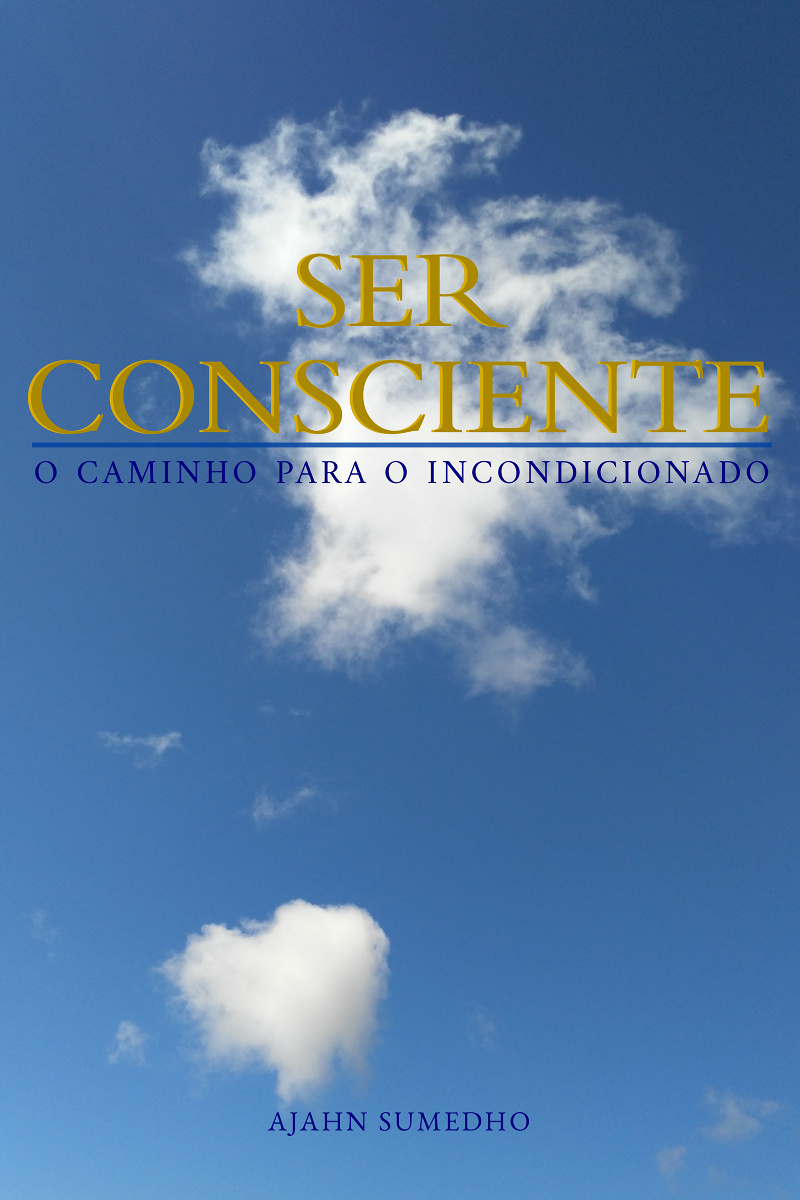
\includegraphics[height=\paperheight]{./desktop-cover.jpg}}
\fi

\cleartorecto
\thispagestyle{empty}
\vspace*{5em}

{\centering

\settowidth{\titleLength}{%
  {\Large\chapterTitleFont\scshape\MakeLowercase{\thetitle}}%
}

{\Large\chapterTitleFont\scshape\MakeLowercase{\thetitle}}\\[0.3\baselineskip]
\setlength{\xheight}{\heightof{X}}
\raisebox{0.5\xheight}{\color[gray]{0.4}\rule{\titleLength}{0.25pt}}\\[0.3\baselineskip]
{\itshape
\thesubtitle}

\vfill

\theauthor

\vspace*{5em}

}



\cleartoverso
\thispagestyle{empty}

{\copyrightsize
\centering
\setlength{\parindent}{0pt}%
\setlength{\parskip}{0.8\baselineskip}%

\thetitle\\
por \theauthor

Publicações Sumedhārāma\\
\href{http://sumedharama.pt}{www.sumedharama.pt}

As publicações de Sumedharama são para distribuição gratuita. Na maioria
dos casos, isto é possível graças a doações, de indivíduos ou grupos,
feitas especificamente para que as publicações dos ensinamentos do
Buddha possam estar disponíveis gratuitamente.

\textit{Sabbadānaṃ dhammadānaṃ jinati}\\
`A oferta de Dhamma é superior a qualquer outra oferta.'

Este livro encontra-se disponível para distribuição gratuita em\\
\href{http://fsbooks.org/}{www.fsbooks.org}

ISBN \theISBN

Copyright \copyright\ Publicações Sumedhārāma 2018

Traduzido por Bhikkhu Appamādo

Tradução autorizada da edição inglesa:

\emph{Mindfulness: The Path to the Deathless}\\
Published by Amaravati Publications, 1987

\vfill

{\footnotesize

Este trabalho está licenciado com uma Licença Creative Commons\\
Atribuição-NãoComercial-SemDerivações 4.0 Internacional.

Veja página \pageref{copyright-details} para mais detalhes sobre direitos e restrições desta licença.

Produzido com o sistema tipográfico \LaTeX.\\
Fonte utilizada: Gentium e Crimson~Roman.

\theEditionInfo

}}


\cleartorecto
\thispagestyle{empty}

\mbox{}\vfill

\begin{verse}

{\itshape
Lorem ipsum dolor sit amet,\\
consectetuer adipiscing elit.
}


\end{verse}

\vfill\mbox{}


\cleartorecto
\tableofcontents*

\chapter{Introdução}

O objectivo deste livro é proporcionar uma instrução clara e uma
reflexão sobre meditação budista, tal como é ensinada por Ajahn Sumedho,
um bhikkhu (monge) da tradição Theravada. Os capítulos seguintes foram
editados a partir de palestras mais longas proferidas por Ajahn Sumedho
a meditadores, como uma abordagem prática à sabedoria do Budismo. Esta
sabedoria é também conhecida como Dhamma.

Somos convidados a usar este livro como um manual, passo"-a-passo.
O primeiro capítulo tenta apresentar uma visão geral da
prática do Budismo e as secções subsequentes podem ser entendidas uma a
uma e seguidas de um período de meditação. O terceiro capítulo é uma
reflexão sobre a compreensão que se desenvolve através da meditação. O
livro termina com a forma de tomar os Refúgios e os Preceitos o que
redimensiona a prática da meditação dentro do contexto mais abrangente
do trabalho a ter com a mente. Estes podem ser pedidos formalmente aos
monásticos budistas (Saṅgha) ou serem assumidos pessoalmente. Eles
constituem os pressupostos através dos quais os valores espirituais são
trazidos ao mundo.

A primeira edição deste livro, em inglês, (2.000 cópias) foi impressa em
1985 -- aquando da abertura do Centro Budista Amarāvatī -- tendo esta se
esgotado rapidamente. O livro foi muito apreciado e algumas pessoas
ofereceram"-se para patrocinar uma nova impressão; desta forma fizemos
uma revisão mais meticulosa do que a anterior e adicionámos algum
design para melhorar o livro como um todo; à parte disso o texto
manteve"-se. Como este livro foi inteiramente produzido através de
contribuições voluntárias e de serviço ao Dhamma, é pedido aos leitores
que respeitem esta oferenda, mantendo"-a disponível de forma gratuita.

Possam todos os seres realizar a Verdade.

\bigskip

{\raggedleft
Venerável Succito\\
Centro Budista Amarāvatī\\
Maio 1986
\par}




\chapter{Antes de começar}

A maior parte destas instruções podem ser levadas a cabo quer estejamos
sentados, em pé ou a andar. Contudo, estar consciente da respiração
(\emph{ānāpānasati}) tal como apresentado nos primeiros capítulos é algo
geralmente realizado na postura de sentado, uma vez que esse trabalho é
potenciado quando realizado num estado físico de quietude e
estabilidade. Para este estado a ênfase é sentarmo"-nos de forma a que a
coluna esteja erguida mas não em esforço, com o pescoço alinhado com a
coluna e a cabeça em equilíbrio de forma a não pender para a frente. É
de opinião geral que a postura de lótus de pernas cruzadas (sentados
numa almofada ou num tapete, com um ou ambos os pés colocados na coxa
oposta, com as plantas dos pés para cima) confere um equilíbrio ideal
entre esforço e estabilidade -- após alguns meses de prática. É bom
treinarmo"-nos gentilmente nesta direcção, um pouco de cada vez. Se esta
postura for muito difícil pode ser usada uma cadeira de costas direitas.

Após ter"-se alcançado estabilidade e um certo equilíbrio físico, a cara
e os braços devem ficar descontraidos, com as mãos a descansar no colo,
uma na palma da outra. Deixem as pálpebras fecharem"-se, relaxem a mente
\ldots{} escolham o objecto de meditação.

\emph{Jongrom}, uma palavra Tailandesa derivada do Pāli (linguagem das
escrituras) `\emph{caṅkama}' significa passear para a frente e para trás
num caminho a direito. O caminho deve ser medido, sendo o ideal vinte a
trinta passos entre dois objectos claramente
identificáveis de modo a não ter que contar os passos enquanto
pratica o \emph{jongrom}. As mãos deverão estar unidas de uma forma
suave, à frente ou atrás do corpo, com os braços relaxados. O olhar
deverá estar direccionado no caminho sem se focar nele, a uma distância
de aproximadamente dez passos à frente, não para observar nada em
particular mas para manter o ângulo mais confortável para o pescoço. O
caminhar começa então com uma postura correcta e quando se chega ao fim
do percurso devemos permanecer imóveis por um período que pode durar uma
ou duas respirações. Então, conscientemente, viramo"-nos e recomeçamos a
andar no sentido contrário.



% Page 1 is the first page of the first chapter.
\mainmatter

\part{Investigação}

\chapter{O que é Meditação?}

A palavra meditação é uma palavra bastante usada nos dias de hoje,
abrangendo um vasto leque de práticas. No Budismo fala-se de dois tipos
de meditação -- `\emph{samatha}' e `\emph{vipassanā}'. A meditação
`\emph{samatha}' é um tipo de meditação na qual se concentra a mente num
objecto não a deixando perambular por outras coisas. Escolhe-se um
objecto de meditação, tal como a percepção da respiração, colocando-se
toda a atenção nas sensações da inalação e da exalação. Através desta
prática começamos eventualmente a experienciar uma mente calma e ficamos
tranquilos, pois estamos a eliminar todas as outras impressões que
captamos através dos sentidos.

Os objectos usados para acalmar a mente são tranquilizadores (nem valia
a pena dizer!). Se quiserem excitar a mente vão para um sítio excitante,
não vão para um mosteiro Budista, mas sim a uma discoteca!... Excitação
é algo no qual é fácil concentrarmo-nos. É uma vibração tão forte que
nos atrai imediatamente. Se formos ao cinema e o filme for realmente
excitante ficamos fixados no ecrã. Não temos que fazer qualquer esforço
para observar algo que é excitante, romântico ou repleto de aventuras.
Mas, não estando acostumados, observar um objecto tranquilizador pode
ser tremendamente enfadonho. Quando estamos habituados a coisas muito
mais excitantes o que é que pode ser mais aborrecido do que ficarmos a
observar a nossa própria respiração? Para o
fazermos temos que `forçar' a nossa mente uma vez que a respiração não é
interessante, romântica, cheia de aventuras ou cintilante -- é
simplesmente o que é. Por isso temos de nos esforçar, pois não estamos a
receber qualquer estímulo vindo do exterior.

Neste tipo de meditação não tentamos criar qualquer imagem, apenas
concentramo-nos na sensação normal do nosso corpo tal como ele está no
momento, mantendo a nossa atenção na respiração. Quando fazemos isto a
respiração torna-se cada vez mais regulada e nós acalmamos\ldots{}
conheço pessoas que prescreveram meditação \emph{samatha} para a tensão
arterial elevada pois acalma o coração.

Assim, esta é a prática da tranquilidade. Podemos escolher diferentes
objectos para nos concentrarmos, mantendo a nossa atenção até sermos
absorvidos ou nos tornarmos um só com o objecto. Na realidade sente-se
uma noção de unidade com o objecto no qual nos concentramos e isto é o
que é chamado de absorção.

A outra prática é `\emph{vipassanā}' ou meditação de \emph{insight}. Com
a meditação de \emph{insight} abrimos a mente para tudo. Não escolhemos
nenhum objecto em particular para nos concentrarmos ou absorvermos, mas
ficamos simplesmente a observar de forma a compreendermos as coisas como
elas são. E o que podemos observar ao ver ``as coisas como são'' é que
toda a experiência sensorial é impermanente. Tudo o que vemos, ouvimos,
cheiramos, saboreamos e tocamos, todas as condições mentais -- os nossos
sentimentos, memórias e pensamentos -- são condições da mente em
constante mudança, as quais surgem e cessam. Em \emph{vipassanā}
assumimos esta característica da impermanência (ou mudança) como uma
forma de olhar para toda a experiência sensorial que podemos observar
enquanto estamos aqui sentados.

Não se trata de uma mera atitude filosófica ou de uma crença numa teoria
budista específica. A impermanência é para ser totalmente reconhecida no
nosso interior através da abertura da mente à observação e
consciencialização da realidade. Não é uma questão de análise, assumindo
que a realidade deveria ser de uma determinada forma e, quando não é,
tentar perceber o porquê. Com a prática de \emph{insight} não estamos
nem a tentar analisar-nos, nem a tentar mudar algo de maneira a que isso
se adeque aos nossos desejos. Nesta prática observamos simplesmente que
tudo aquilo que surge, seja mental ou físico, passa e desaparece.

Isto inclui os próprios órgãos dos sentidos, o objecto dos sentidos e a
consciência que surge aquando do contacto com esses objectos. Existem
também as condições mentais de gostar e de não gostar do que vemos,
cheiramos, saboreamos, sentimos ou tocamos; os nomes que atribuímos e as
ideias, palavras e conceitos que criamos à volta da experiência
sensorial. Grande parte da nossa vida é baseada em assunções feitas
devido a não se compreender e a não se investigar verdadeiramente a
realidade, tal qual como é. A vida, para quem não está desperto nem
consciente, pode tornar-se deprimente ou confusa, especialmente quando
algo nos decepciona ou quando ocorre alguma tragédia. Nessas alturas
ficamos esmagados por não observamos a realidade do momento.

Na terminologia budista usamos a palavra Dhamma, ou Dharma, que
significa, `leis naturais'. Quando observamos e praticamos o Dhamma
abrimos a nossa mente para a realidade. Desta forma já não estamos a
reagir cegamente à experiência dos sentidos mas sim a compreendê-la e,
através dessa compreensão, chegamos ao desapego. Começamos a
libertarmo-nos de ser naturalmente esmagados, cegos e iludidos pelas
aparências. Estar consciente e desperto não é uma questão de nos
\emph{tornarmos} nisso, mas de o \emph{sermos}.

Observemos as coisas tal como elas são neste preciso momento ao invés de
fazermos algo agora para nos tornarmos conscientes no futuro. Observamos
o corpo como ele é, aqui sentado. Não pertence tudo à natureza? O corpo
humano pertence à terra, precisa de ser sustentado por coisas
provenientes da terra. Não podemos viver simplesmente do ar nem tentar
importar comida de Marte ou de Vénus. Temos que comer do que vive e
cresce nesta Terra. Quando o corpo morre regressa à terra, apodrece,
desfaz-se e torna-se novamente um com a terra. Segue as leis da
natureza, da criação e da destruição, do nascimento e da morte. Tudo o
que nasce não se mantém no mesmo estado: cresce, envelhece e morre. Tudo
na natureza, até o próprio universo, tem os seus períodos de existência,
nascimento e morte, começo e fim. Tudo aquilo de que nos apercebemos e
que concebemos é transitório, impermanente, e portanto nunca nos poderá
satisfazer de forma permanente.

Na prática do Dhamma também podemos observar o carácter insatisfatório
da experiência sensorial. Reparem simplesmente na vossa própria vida:
quando esperam satisfazer-se através de objectos ou experiências
sensoriais, apenas o conseguem fazer temporariamente, talvez
gratificados e felizes nesse momento, mas imediatamente a seguir isso
muda. Isto acontece por não existir nada na consciência sensitiva que
tenha essência ou qualidade permanente, daí a experiência sensorial ser
uma constante mudança. Devido à ignorância e à falta de compreensão
dependemos imenso dessa experiência; habituamo-nos a exigir, desejar e a
criar todo o tipo de coisas, apenas para de seguida nos sentirmos
terrivelmente desapontados, desesperados, pesarosos e assustados. Essas
mesmas expectativas e esperanças levam-nos ao desespero, à angústia, à
lástima, à dor, ao lamento, à velhice, à doença e à morte.

Esta é a forma de examinar a consciência sensorial. A mente pode pensar
de forma abstracta, pode criar todo o tipo de ideias e imagens, pode
criar coisas muito apuradas ou grosseiras. Existe toda uma gama de
possibilidades desde estados muito aperfeiçoados de graça, felicidade e
êxtase até às mais densas e dolorosas misérias: do céu ao inferno,
usando uma terminologia mais pitoresca. Mas não existe nenhum Inferno
permanente nem nenhum Céu permanente. Na verdade não existe nenhum
estado permanente que possa ser concebido ou criado. Ao meditarmos,
assim que começamos a perceber as limitações, a qualidade insatisfatória
e a natureza transitória de toda a experiência sensorial, também
começamos a perceber que isto não é o eu ou o meu, é `\emph{anattā}',
`não-eu'.

Quando tal é realizado começamos a libertar-nos da identificação com as
condições sensoriais. Isto acontece não por as rejeitarmos, mas por as
compreendermos tal como elas são. Trata-se de uma verdade a ser
realizada, não de uma crença. `\emph{Anattā}' não é uma crença budista
mas sim uma realização. Mas se não despendermos algum tempo da nossa
vida a tentar investigar e compreender, iremos provavelmente viver
sempre na convicção de que somos o nosso corpo. Podemos a dada altura
pensar `Oh, eu não sou o meu corpo' por termos lido alguma poesia
inspiradora ou uma nova abordagem filosófica, podemos até achar que é
uma boa ideia não se ser o corpo, mas ainda não realizámos isso. Alguns
intelectuais podem dizer `Nós não somos o corpo, o corpo não é o eu' --
dizê-lo é fácil, mas sabê-lo realmente é outra coisa. Através desta
prática de meditação, da investigação e compreensão da realidade,
começamos a libertarmo-nos do apego. Quando já não tivermos expectativas
ou exigências então, obviamente, já não iremos sentir o desespero, a
pena e a angústia resultantes de quando não conseguimos aquilo que
queremos. Este é, de facto, o objectivo
-- `\emph{Nibbāna}' ou a realização de não nos agarrarmos a nenhum
fenómeno que tenha um princípio e um fim. Quando abrimos mão deste
habitual e insidioso apego a tudo quanto nasce e morre, começamos a
realizar a `não-morte'.

Algumas pessoas vivem simplesmente reagindo à vida porque foram
condicionadas a fazê-lo, como os cães de Pavlov. Se não estivermos
despertos para as coisas tal como elas são, então, na verdade, não somos
mais que uma mera criatura inteligente condicionada semelhante a um
ignorante cão condicionado. Podemos olhar com ar de superioridade para o
cão de Pavlov que saliva quando a campainha toca, mas reparem como
fazemos coisas tão semelhantes. Isto deve-se ao facto de que na
experiência sensorial tudo é condicionante, não se trata de ser pessoa,
alma ou essência pessoal. Estes corpos, sentimentos, memórias e
pensamentos são percepções condicionadas na mente através da dor, devido
a termos nascido como seres humanos, nas nossas respectivas famílias,
classe social, raça, nacionalidade, etc.; dependendo se temos um corpo
masculino ou feminino, atraente ou não, \ldots{} e por aí adiante. Tudo
isto são apenas condições que não são nossas, que não somos nós. Estas
condições obedecem às leis da natureza, as leis naturais. Não podemos
dizer `Não quero que o meu corpo envelheça.' Bem, podemos dizê-lo mas,
não importa o quão insistentes sejamos, o corpo continuará a envelhecer.
Não podemos esperar que o corpo nunca adoeça ou sinta dor ou ainda que
tenha sempre visão e audição perfeitas. Gostaríamos, não é verdade? `Eu
espero ser sempre saudável. Nunca serei um inválido e terei sempre uma
boa visão, nunca ficarei cego; tenho bom ouvido e por isso nunca serei
uma daquelas pessoas de idade para as quais os outros têm de gritar e
nunca ficarei senil e terei sempre controlo das minhas faculdades até
morrer aos noventa e cinco anos de idade, completamente desperto, com a
mente clara e alegre. E morrerei naturalmente enquanto durmo, sem dor.'
Isto é como todos gostaríamos que fosse. Até pode ser que, de entre nós,
alguns continuem a viver por bastante tempo e morram de forma bastante
edílica ou também pode acontecer que amanhã
os nossos olhos saltem das órbitas! Não é muito provável mas pode
acontecer! Contudo, o fardo da vida diminui consideravelmente quando
reflectimos nas limitações da nossa própria vida. Aí sabemos o que
podemos alcançar, o que podemos aprender. Tanta miséria humana resulta
de criarmos demasiadas expectativas e nunca sermos capazes de alcançar
tudo aquilo que desejamos.

Na nossa meditação e compreensão intuitiva das coisas tal como elas são,
vemos que beleza, refinamento e prazer são condições impermanentes --
assim como a dor, miséria e feiúra. Se conseguirmos realmente
compreender isso, poderemos desfrutar e aguentar o que quer que seja que
nos aconteça. Na verdade, grande parte da lição da vida consiste em
aprender a suportar aquilo que não gostamos em nós próprios e no mundo à
nossa volta; sermos capazes de ser pacientes e calmos, e não fazermos um
drama acerca das imperfeições da experiência sensorial. Podemo-nos
adaptar, suportar e aceitar as características mutáveis do ciclo do
nascimento e da morte através do ``abrir mão'' e do desapego a esse
mesmo ciclo. Quando nos libertamos dessa identificação, experienciamos a
nossa verdadeira natureza, a qual é brilhante, clara, sábia, mas que já
não é algo pessoal, não é `eu' ou `meu' -- não existem metas nem apegos.
Apenas nos podemos apegar àquilo que não é a nossa consciência pura!

Os ensinamentos do Buddha são simples meios úteis, formas de observar a
experiência sensorial que nos ajudam a compreendê-la. Não são
mandamentos ou dogmas religiosos nos quais temos de acreditar e aceitar.
São meras linhas guias que apontam para a maneira como as coisas são.
Desta forma não estamos a usar os ensinamentos do Buddha apegando-nos a
eles como um fim em si próprio, mas apenas para nos relembrarmos de
estar despertos, alertas e conscientes de que tudo o que surge, cessa.

Trata-se de uma observação e reflexão contínua e constante do mundo
sensitivo, visto este exercer uma influência forte e poderosa. Vivendo
num corpo assim, na sociedade actual, as pressões em todos nós são
incríveis. Tudo se move tão rapidamente -- a televisão e a tecnologia
desta era, os carros -- tudo tende a mover-se a um ritmo muito rápido. É
tudo muito atraente, excitante e interessante, e tudo atrai os nossos
sentidos para o exterior. Simplesmente reparemos, quando vamos a
Londres, como toda a publicidade chama a nossa atenção para os cigarros
e garrafas de whisky! A nossa atenção é levada para coisas que podemos
comprar, reafirmando o renascer na experiência sensorial. A sociedade
materialista estimula a avidez de forma a gastarmos dinheiro e ainda
assim a nunca estarmos contentes com o que temos. Existe sempre algo
melhor, mais recente \ldots{} mais delicioso do que aquilo que ontem era
o mais delicioso \ldots{} e continua e continua, puxando-nos
exteriormente para os objectos dos sentidos.

Mas na sala de meditação, não vimos aqui para olhar uns para os outros
ou para sermos levados ou atraídos para qualquer um dos objectos na
sala, mas para os usar de forma a relembrar. Somos relembrados quer a
concentrar as nossas mentes num objecto pacífico quer a abrir a mente a
investigar e a reflectir sobre a realidade. Cada um tem de experienciar
isto por si próprio. Não é a iluminação de alguém que vai iluminar os
restantes. Este é um movimento para o interior; não é o olhar para fora,
para alguém que é iluminado, que nos ilumina. Damos esta oportunidade de
encorajamento e encaminhamento para que aqueles que estão interessados o
possam realizar. Aqui podemos, a maior parte do tempo, ter a certeza de
que ninguém
nos vai roubar a mala! Hoje em dia não podemos confiar em
nada, mas o risco disso acontecer aqui é menor do que se tivéssemos
sentados em Piccadilly Circus. Os mosteiros Budistas são refúgios para
este tipo de abertura da mente. Esta é a nossa oportunidade enquanto
seres humanos. Como seres humanos temos uma mente que pode reflectir e
observar. Podemos observar, quer estejamos felizes ou miseráveis.
Podemos observar o ódio, o ciúme ou a confusão na nossa mente. Quando
estamos sentados e sentimo-nos realmente confusos e aborrecidos existe
algo em nós que o sabe. Podemos odiar e reagir cegamente contra isso,
mas se formos mais pacientes conseguimos observar que isso é uma
condição temporária e transiente de confusão, ódio ou avareza. Mas um
animal não consegue fazer isso. Quando está zangado ele é somente isso,
perdidamente. Digam a um gato zangado para observar a sua raiva! Eu
nunca consegui ir muito longe com a nossa gata, ela não consegue
reflectir sobre a gula. Mas eu consigo e tenho a certeza de que todos
vocês também o conseguem fazer. Quando vemos comida deliciosa à nossa
frente o movimento da mente é o mesmo da nossa gata Doris. Mas nós
conseguimos observar a atracção animal para coisas que parecem boas e
que cheiram bem.

Quando observamos e compreendemos o impulso estamos a usar sabedoria.
Aquilo que observa a gula não é gula. A gula não se pode observar a ela
mesma, mas aquilo que não é gula pode observá-la. Este observar é aquilo
a que chamamos `Buddha' ou
`Sabedoria de Buddha' -- a consciência das coisas tal como são na
realidade.
\part{Instrução}

\chapter{Observando a Respiração (Ānāpānasati)}

\emph{Ānāpānasati} é a prática de ancorar a mente na respiração. Quer
sejamos já peritos ou quer tenhamos desistido da prática por nos
considerarmos um caso perdido, existe sempre um tempinho para observar a
respiração. É uma oportunidade para desenvolver ``samādhi''
(concentração) colocando toda a nossa atenção exclusivamente na sensação
da respiração. Nesse momento comprometam"-se totalmente nesse ponto único
durante uma inspiração, e depois durante uma expiração. Não tentem fazer,
quinze minutos pois nunca seriam bem sucedidos se esse fosse o período
de tempo designado para se focarem num só ponto. Portanto usem esta
duração de tempo de uma inspiração e de uma expiração.

O sucesso disto depende mais da vossa paciência do que da vossa vontade,
pois a mente vagueia e temos sempre que, pacientemente, voltar à
respiração. Quando estamos conscientes de que a mente está a vaguear
então reparamos no que se passa: pode dever"-se ao facto de colocarmos
muita energia no princípio e depois não a conseguimos manter e
controlar. Estamos assim a usar a duração de tempo de uma inspiração e de
uma expiração de modo a limitar o esforço apenas este período de tempo,
durante o qual mantemos a nossa atenção. Empenhem"-se em colocar um
esforço no princípio da inspiração e em mantê"-lo. Depois façam o
mesmo durante a expiração e de novo na inspiração. Eventualmente tudo se
torna estável e diz"-se que estamos em \emph{samādhi} quando já não
precisamos aplicar esforço. De princípio parece ser um esforço enorme ou
parece que não o conseguimos fazer por não termos esse hábito. A maioria
das mentes foi treinada para usar o pensamento associativo, para ler
livros, para ir de palavra em palavra, para ter pensamentos e conceitos
baseados na razão e na lógica. Contudo, \emph{ānāpānasati} é um tipo
diferente de treino onde o objecto no qual nos concentramos é tão
simples que não oferece qualquer interesse a nível intelectual. Não se
trata de uma questão de se estar interessado, mas de aplicar esforço e
de usar esta função natural do corpo como um ponto de concentração. O
corpo respira, quer estejamos cientes disso ou não. Não é como
\emph{prāṇāyama}, em que estamos a desenvolver poder através da
respiração. Aqui estamos a desenvolver samādhi' -- concentração -- e um
estado consciente através da observação da respiração, tal como ela é no
momento. Como qualquer outra coisa, isto é algo que temos de praticar
para o podermos fazer; ninguém tem problema algum em perceber a teoria,
mas é a prática contínua dessa teoria que faz com que as pessoas se
sintam desencorajadas.

Mas reparem nesse desencorajamento, que surge por não sermos capazes de
obter o resultado que desejamos, pois ele é o obstáculo para a prática.
Reparem bem nesse mesmo sentimento, reconheçam"-no e depois deixem"-no ir.
Voltem novamente à respiração. Estejam conscientes desse momento em que
se sentem fartos ou sentem aversão ou impaciência, reconheçam"-no,
deixem"-no ir, e voltem de novo à respiração.

\chapter{O Mantra `Buddho'}

% TODO review: yellow highlight: som `\emph{Bud}' formal

Se tiverem uma mente pensante muito activa, talvez possam achar o
mantra\footnote{%
  \emph{mantra}: palavra de relevância religiosa. A repetição de mantras pode
  ser utilizada como objecto de meditação.}
`\emph{Buddho}' algo de grande ajuda. Inalem em `\emph{Bud}' e
exalem em `\emph{dho}' de forma a pensarem nisso em cada inalação. Isto
é uma maneira de se manter a concentração: durante os próximos quinze
minutos façam a \emph{ānāpānasati}, colocando toda a vossa atenção,
aquietando a vossa mente com o som mântrico `\emph{Bud"-dho}'. Aprendam a
treinar a mente até terem clareza e lucidez mental em vez de se
afundarem em passividade. Isto requer esforço contínuo: uma inspiração de
`\emph{Bud}' completamente clara na vossa mente, o próprio pensamento
presente e claro desde o princípio até ao fim da inspiração. E
`\emph{dho}' na expiração. Nessa altura larguem tudo o resto. Esta agora
é a ocasião para fazermos exclusivamente isto -- podemos resolver os
nossos problemas e os problemas do mundo a seguir. Neste momento só nos
é pedido isto. Tragam o mantra à consciência. Tornem"-se completamente
conscientes do mantra em vez deste ser apenas uma formalidade passiva
que deixa a mente dormente; energizem a mente de forma a que a inspiração
em `\emph{Bud}' seja uma inspiração lúcida, não apenas um som `\emph{Bud}'
formal que vai desaparecendo por nunca ter sido avivado ou refrescado
pelas nossas mentes. Podem visualizá"-lo ortograficamente para terem essa
sílaba completamente presente durante o período de uma inspiração, do
princípio ao fim. Durante a expiração `\emph{dho}' pode ser realizado da
mesma forma, até haver uma continuidade de esforço ao invés de
esporádicas tentativas, começos e fracassos.

Verifiquem se de seguida surgem alguns pensamentos obsessivos -- alguma
frase tola que talvez esteja a passar pela vossa mente. Se se deixarem
naturalmente afundar num estado passivo, então os pensamentos obsessivos
irão tomar conta da mente. Mas ao aprenderem como a mente funciona e a
usá"-la habilmente, podem ter este particular pensamento, o conceito de
`\emph{Buddho}' (o Buddha, aquele que sabe) e sustê"-lo na vossa mente
como um pensamento comum obsessivo, mas como um uso saudável da
capacidade pensante, para manter a concentração durante o período de uma
inspiração - expiração, durante quinze minutos.

A prática é essa, independentemente de quantas vezes falharem e a mente
começar a vaguear, somente têm de reparar que estão distraídos, ou que
estão a pensar nisso ou que prefeririam não se importar com
`\emph{Buddho}' -- `Eu não quero fazer isto. Prefiro somente sentar"-me
aqui e relaxar e não ter que fazer nenhum esforço. Não sinto vontade de
o fazer.' Ou talvez tenham outras coisas na vossa mente nesta altura,
surgindo furtivamente no limiar da consciência -- reparem nisso.
Verifiquem que estado de ânimo está presente na vossa mente nesse
preciso momento -- não de forma crítica ou desencorajadora mas, calma e
descontraidamente, reparem se isso vos tranquiliza ou se se sentem
letárgicos e sonolentos; se estiveram a pensar durante todo esse tempo
ou se estiveram a concentrar"-se. Apenas para estarem cientes.

O obstáculo para a prática da concentração é a rejeição ao fracasso e o
incrível desejo de sucesso. A prática não é uma questão de força de
vontade mas de sabedoria, de reconhecer a sabedoria. Com esta prática
podem aprender onde estão as vossas fraquezas, onde é que se perdem.
Testemunhem o tipo de características de personalidade que desenvolveram
na vossa vida até esta altura, não para serem críticos mas para saberem
como lidar com elas sem serem escravos das mesmas. Isto significa
uma cuidadosa e sábia reflexão sobre a realidade. Por isso observem e
reconheçam até os mais horríveis e confusos estados mentais, em vez de
evitá"-los a todo o custo. Essa é uma qualidade de persistência.
`\emph{Nibbāna}'\footnote{%
  \emph{Nibbāna}: Paz através do desapego, também se pode escrever `Nirvāņa'.}
é muitas vezes descrita como sendo `\emph{cool}'
(fresca). Parece conversa de hippy, não é? Mas o significado dessa
palavra tem um certo sentido. Frescura em termos de quê? No sentido de
que é refrescante por não ser emaranhada em paixões mas sim desapegada,
alerta e equilibrada.

A palavra `\emph{Buddho}' é uma palavra que podem desenvolver nas vossas
vidas como algo para preencher a mente em vez de preocupações e todo o
tipo de hábitos pouco saudáveis. Peguem na palavra, olhem para ela,
escutem"-na: `\emph{Buddho}'! Significa aquele que sabe, o Buddha, o
desperto, aquele que é desperto. Podem visualizar na vossa mente. Ouçam
o que a vossa mente diz: blá, blá, blá\ldots{} continuamente por aí
fora, um infindável tipo de excremento de aversões e medos reprimidos.
Estão agora então, a reconhecer isso. Não estamos a usar a palavra
`\emph{Bud- dho}' como um cassetete para aniquilar ou reprimir coisas,
mas como um meio inteligente. Podemos usar as mais requintadas
ferramentas para matar e prejudicar os outros, não podemos? Podemos
agarrar na mais bela estátua do Buddha e esmagar a cabeça de alguém com
ela! Isso não seria aquilo a que chamamos
`\emph{Buddhanussati}', Reflexão no Buddha! Mas talvez façamos isso com
a palavra `Buddho' de forma a suprimir esses pensamentos ou sentimentos.
Isso não é fazer um uso inteligente da palavra. Lembremo"-nos que não
estamos aqui para aniquilar, mas para permitir que as coisas se
desvaneçam. Trata"-se de uma prática gentil de pacientemente impor
`\emph{Buddho}' sobre o pensamento, não por exasperação, mas de uma
forma firme e deliberada.

O mundo precisa de aprender a fazer isto, não é? Os Estados Unidos e a
União Soviética poderiam fazê"-lo ao invés de agarrarem em metralhadoras
e armas nucleares e aniquilarem coisas que se lhes intrometem no
caminho, ou dizerem coisas horríveis e ofensivas uns aos outros. Até nas
nossas vidas nós fazemos isso, não fazemos? Quantos de vocês disseram
coisas desagradáveis a alguém recentemente, coisas que magoam,
criticismo descortês e ofensivo, simplesmente porque a outra pessoa vos
irrita, empata ou assusta? Pratiquemos então com as pequenas coisas
irritantes e desagradáveis que estão na nossa mente, coisas que são
tolas e estúpidas. Usemos `\emph{Buddho}' não como um cassetete mas como
um meio inteligente de permitir que esses pensamentos sigam o seu rumo;
como um meio para os largarmos. Agora, durante os próximos quinze
minutos, voltem aos vossos narizes, com o mantra `\emph{Buddho}'. Vejam
como usá"-lo e trabalhar com ele.

\chapter{Esforço e Relaxamento}

Esforço é simplesmente fazer aquilo que temos que fazer. Varia de acordo
com as características e hábitos de cada um. Algumas pessoas têm muita
energia -- tanta que estão sempre a mexer, à procura de coisas para
fazer. Vemo"-las o tempo todo a tentar encontrar coisas para fazer,
colocando tudo no exterior. Na meditação não estamos à procura de algo
para fazer como um escape, mas estamos a desenvolver um tipo de esforço
interno. Observamos a mente e concentramo"-nos no assunto.

Se fizerem demasiado esforço apenas ficarão agitados, e se não fizerem
esforço suficiente ficam entorpecidos e o corpo amolece. O nosso corpo é
algo muito bom para ter em atenção no que diz respeito ao esforço:
colocar o corpo direito, alinhá"-lo, pôr o peito para fora, manter a
coluna vertebral direita, tudo isto requer muita força de vontade. Se
estiverem demasiado moles irão simplesmente encontrar a postura mais
fácil -- a força da gravidade puxa"-vos para baixo. Quando está frio têm
de puxar a energia para cima através da coluna de maneira a aquecerem o
vosso corpo ao invés de se enfiarem debaixo de cobertores.

Com `\emph{ānāpānasati}', a `ter a respiração como uma âncora para a
consciência', concentram"-se no ritmo. Considero isso muito útil para
aprender a acalmar em vez de fazer tudo rapidamente -- tal como pensar;
estão"-se a concentrar num ritmo que é muito mais lento que os vossos
pensamentos. Mas \emph{ānāpānasati} requer que abrandem pois tem um
ritmo bastante lento que faz com que tal aconteça. Paramos de pensar.
Estamos contentes com uma inspiração, uma expiração\ldots{} temos todo o
tempo do mundo, só para ficar com uma inspiração, desde o princípio ao
fim.

Se estiverem a tentar alcançar \emph{samādhi}' através de
\emph{ānāpānasati}, então já estabeleceram a si próprios um objectivo --
estão a fazê"-lo para obterem algo para vós e, então, \emph{ānāpānasati}
torna"-se uma experiência muito frustrante e ficam zangados com isso.
Será que podem estar somente com uma inspiração? Estar satisfeitos com uma
simples expiração? Estar satisfeitos apenas com o breve espaço de tempo
que têm para se acalmarem?

Quando pretendem alcançar \emph{jhānas} (absorções) a partir desta
meditação e realmente colocam bastante esforço nisso, não acalmam. Estão
a tentar alcançar ou a obter algo, ao invés de humildemente ficarem
satisfeitos com uma respiração. O sucesso de \emph{ānāpānasati} é
simplesmente esse -- estar consciente durante uma inspiração, durante o
período de tempo de uma inspiração. Estabeleçam a vossa atenção no
princípio e no fim -- ou no princípio, meio e fim. Isto dá"-vos alguns
pontos definidos para reflexão de maneira a que, se a mente vagueia
imenso durante a prática, possam tomar especial atenção, escrutinando o
princípio, o meio e o fim. Se não o fizerem a mente voltará a vaguear.

Todo o nosso esforço vai para aí; tudo o resto é suprimido durante esse
tempo, ou descartado. Reflictam na diferença entre inspiração e
expiração -- examinem"-na. De qual é que gostam mais? Por vezes a
respiração parece que vai desaparecer, tornando"-se muito rarefeita. O
corpo parece respirar por si próprio e têm este estranho sentimento de
que não vão respirar. É um pouco assustador.

Mas isto é um exercício; centrem"-se na respiração, sem a controlarem de
todo. Por vezes quando se concentram nas narinas, sentem que todo o
corpo está a respirar. O corpo continua a respirar por si próprio.

Por vezes levamos as coisas demasiado a sério, com uma total falta de
alegria e felicidade, sem sentido de humor, apenas
reprimindo tudo. Alegrem a mente, estejam descontraídos e à
vontade, tenham todo o tempo do mundo sem a pressão de terem de alcançar
algo importante: nada de especial, nada para atingir. Trata"-se de algo
simples, mesmo quando fazem apenas uma inspiração conscientemente
durante a manhã, isso é melhor do que o que a maior parte das pessoas
está a fazer e de certeza que é melhor do que estar sempre disperso.

Se forem muito negativos devem tentar ser alguém agradável e com uma
maior auto"-aceitação. Relaxem e não façam da meditação uma tarefa
pesada. Vejam"-na como uma oportunidade para estar em paz e à vontade com
o momento presente. Descontraiam o corpo e estejam em paz.

Não estão a batalhar com as forças do mal. Se sentirem aversão para com
\emph{ānāpānasati}, reparem nisso. Não sintam que é algo que têm de
fazer, mas vejam"-na como um prazer, como algo que realmente gostam de
fazer. Não têm de fazer mais nada, podem simplesmente estar
perfeitamente descontraídos. Têm tudo o que precisam; têm a vossa
respiração, têm apenas de se sentar aqui, não há nada difícil para
fazer, não precisam de capacidades especiais, não precisam nem mesmo de
ser particularmente inteligentes. Quando pensam `Eu não consigo fazê"-lo'
reconheçam isso como uma mera resistência, medo ou frustração, e
descontraiam.

Se se sentirem muito tensos e rígidos por causa de \emph{ānāpānasati},
então não o façam. Não façam disso uma coisa difícil, não a tornem numa
tarefa penosa. Se não o conseguirem fazer, então sentem"-se,
simplesmente. Quando eu costumava entrar em esta- dos terríveis eu
apenas contemplava `paz'. Começava a pensar:

`Eu tenho de\ldots{} Eu tenho de\ldots{} Eu tenho de fazer isto.' Então
pensava: `Fica simplesmente em paz, relaxa.'

Dúvida e inquietação, descontentamento e aversão -- rapida- mente
reflectia na palavra paz, dizendo"-a uma e outra vez, hipnotizando"-me,
`relaxa, relaxa'. As dúvidas pessoais começavam a vir:

`Não estou a chegar a lugar nenhum com isto, é inútil, eu quero
obter algo.' Mas logo ficava em paz com isso. Conseguimo"-nos acalmar e
quando descontraímos, conseguimos fazer \emph{ānāpānasati}. Se querem
fazer alguma coisa, então façam \emph{ānāpānasati}.

No princípio a prática pode ser muito aborrecida, sentimo-nos
desesperadamente desajeitados tal como quando estamos a aprender a tocar
guitarra. Quando se começa a tocar, os nossos dedos são desajeitados. É
desesperante! Mas após algum tempo de prática ganha"-se habilidade e
torna"-se bastante fácil. Estamos a aprender a testemunhar o que se passa
na nossa mente para sabermos quando começamos a ficar agitados e tensos,
com aversão a tudo. Reconhecendo isso, não tentamos convencer"-nos de que
é de outra maneira. Estamos completamente conscientes das coisas tal
como elas são: e o que fazemos quando estamos tensos e nervosos?
Descontraímos.

Nos meus primeiros anos com Ajahn Chah, por vezes eu era muito sério no
que respeitava à meditação chegando mesmo a ser demasiado solene e
taciturno comigo próprio. Eu chegava a perder todo o sentido de humor e
a ficar `sério de morte', completamente rígido como um velho tronco.
Costumava fazer imenso esforço, mas tornava"-se tão doloroso e
desagradável pensar `Tenho de\ldots{}sou tão preguiçoso'. Sentia"-me tão
terrivelmente culpado se não passasse o tempo todo a meditar -- um
escuro estado mental desprovido de alegria. Passei a observar isso,
meditando vendo"-me como um ramo seco. Quando tudo se tornava
completamente insuportável eu recordava"-me do oposto: `Não tens de fazer
nada. Nenhum sítio para onde ir, não há nada para ser feito. Está em paz
com a forma como as coisas são agora, descontrai, deixa.' Passei a usar
isto.

Quando a vossa mente se encontra nesta condição, apliquem o oposto,
aprendam a levar as coisas de uma forma suave. Vocês lêem livros acerca
de não fazer esforço algum -- `deixem apenas
acontecer de uma forma natural' -- e pensem `tudo o que tenho de
fazer é ser preguiçoso'. O que acontece é que normalmente caem num
estado entorpecido e passivo. Mas é precisamente nessa altura que
precisam de se esforçar um pouco mais.

Com \emph{ānāpānasati} podem manter o esforço durante uma inspiração. E
se não poderem sustê"-lo durante uma inspiração então façam"-no durante
pelo menos meia inspiração. Desta maneira não estão a tentar ser
perfeitos imediatamente. Não têm de fazer tudo certinho devido a alguma
ideia de como poderia ser, mas trabalhem com os respectivos tipos de
problemas, tal como eles são. Se tivermos uma mente muito dispersa é
sábio reconhecer"-se que assim é -- isso é um \emph{insight}, uma
realização. Pensar que não deveriam ser assim, detestarem"-se ou
sentirem"-se desencorajados por serem de determinada maneira, isso sim, é
ignorância.

Com \emph{ānāpānasati} reconhecem a realidade do agora e partem desse
ponto: sustenham a vossa atenção por um pouco mais de tempo e começam a
perceber o que é a concentração, tomando decisões que podem manter. Não
decisões de Super"-homem quando não são o Super"-homem. Façam
\emph{ānāpānasati} por dez ou quinze minutos em vez de pensar que o
conseguem fazer a noite toda. `Vou fazer \emph{ānāpānasati} desde agora
até ao amanhecer'. Aí falham e aborrecem"-se. Estabeleçam períodos que
sabem que vão conseguir cumprir. Experimentem, trabalhem com a mente até
perceberem como aplicar esforço e como relaxar.

\emph{Ānāpānasati} é algo imediato. Leva"-nos à realização (\emph{in-
sight}) -- \emph{vipassanā}. A natureza impermanente da respiração não é
nossa, ou é? Tendo nascido, o corpo respira por si próprio. Inspiração e
expiração -- uma condiciona a outra. Enquanto o corpo estiver vivo é
assim que será. Não controlamos nada. Respirar pertence à natureza, não
a nós; é não"-eu. Quando observamos isto estamos a fazer
\emph{vipassanā}. Não é algo excitante ou fascinante ou desagradável. É
natural.

\chapter{Caminhando Conscientemente (Jongrom)}

O Caminhar em \emph{`Jongrom'}\footnote{%
  \emph{Jongrom} (palavra tailandesa): andar para a frente e para trás num
  caminho a direito. Ver pág. 2 (FIXME:pageref)}
é uma prática de caminhar centrados no
movimento dos pés. Trazemos a atenção para o caminhar do corpo desde o
princípio de determinado percurso, até ao fim. Damos meia volta e
paramos. Surge então a intenção de andar e assim o fazemos. Reparem no
meio do caminho e no fim, parando, virando, ficando parado; os momentos
em que acalmamos a mente quando esta começa a divagar em todas as
direcções. Se não tivermos cautela podemos planear uma revolução ou algo
assim enquanto fazemos \emph{jongrom}! Quantas revoluções terão sido
planeadas durante \emph{jongrom}\ldots{}? Então em vez de fazer coisas
como essas usamos esse tempo para nos concentrarmos naquilo que na
verdade está a acontecer. Não são sensações fantásticas, mas sim tão
comuns que nem reparamos nelas. Reparem que é preciso esforço para estar
verdadeiramente consciente de coisas assim.

Quando a mente vagueia e dão por vós na Índia enquanto estão a meio do
caminho do \emph{jongrom}, então reconheçam -- `Oh!'
-- nesse momento estão despertos e por isso podem restabelecer a vossa
mente no que está realmente a acontecer, o corpo a andar de um ponto
para o outro. É um treino de paciência pois a mente vagueia por todo o
lado. Se no passado tiveram momentos de graça enquanto faziam
\emph{jongrom} e pensarem `no último retiro fiz meditação andando e
realmente senti apenas o corpo a andar;
senti que não havia `eu' e foi maravilhoso, oh, se o pudesse fazer de
novo\ldots{}' observem então esse desejo de obter algo de acordo com uma
memória de um momento feliz. Reparem nisso como uma condição pois isso é
um obstáculo. Abram mão de tudo, não importa se daí resultará um momento
de graça ou não. Apenas um passo e depois um novo passo -- isso é tudo o
que é preciso, um deixar ir, um ficar satisfeito com pouco em vez de
tentarem obter um estado de graça que talvez tenha acontecido a dada
altura, durante este tipo de meditação. Quanto mais tentarem pior ficará
a vossa mente pois estão a perseguir o desejo de ter uma determinada
experiência maravilhosa, de acordo com a vossa memória. Fiquem
satisfeitos com as coisas como elas são neste momento, em vez de se
precipitarem a fazer algo para obterem determinado estado desejado.

Um passo de cada vez -- reparem quão pacífico é fazer meditação andando,
quando tudo o que temos de fazer é estar presentes em cada passo. Mas se
pensarmos que temos de desenvolver \emph{samādhi}' através desta prática
e a nossa mente viajar em todas as direcções, o que é que acontece? `Eu
não suporto este tipo de meditação, não alcanço nenhuma paz com ela;
tenho praticado tentando ter este sentimento de `andar sem ninguém
andar' e a minha mente simplesmente vagueia por toda a parte' -- isto
acontece porque ainda não percebemos como fazê"-lo; a nossa mente está a
idealizar, a tentar obter algo ao invés de simplesmente ser. Quando
estamos a andar tudo o que temos de fazer é andar. Um passo, um próximo
passo -- simples\ldots{} Mas não é fácil, não é? A mente é distraída,
tentando perceber o que deveríamos estar a fazer, o que está errado
connosco e porque não o conseguimos fazer.

Mas no mosteiro o que fazemos é levantarmo"-nos de manhã, fazer os
cânticos, meditar, sentar, limpar o mosteiro, preparar a
comida, sentar, levantar, andar, trabalhar,\ldots{} o que quer que
seja, simplesmente fazemos aquilo que surge para fazer, uma coisa de cada vez.
Então, estar com as coisas como elas são é desapego, é isso que traz paz
e alívio. A vida muda e podemos observá"-la a mudar, podemo"-nos adaptar à
mudança do mundo dos sentidos, qualquer que seja. Seja agradável ou
desagradável, podemos sempre aguentar e colaborar com a vida, aconteça o
que acontecer. Se realizarmos a verdade, realizamos a paz interior.

\chapter{Amor Incondicional (Mettā)}

Em inglês a palavra `love' (amor) refere"-se a `algo de que gostamos'.
Por exemplo `gosto de arroz pegajoso'\footnote{%
  \emph{sticky rice}: `arroz pegajoso' -- consiste num tipo de arroz
  glutinoso que após cozinhado torna"-se translúcido e pegajoso. Este é um
  prato básico do dia"-a-dia das populações do norte e nordeste tailandês,
  sendo tradicionalmente comido à mão.},
`gosto de manga doce'. Na
verdade quer dizer que gostamos dessas coisas. Gostar é estar apegado a
algo como por exemplo a certa comida que apreciamos ou adoramos. Não a
amamos. \emph{Mettā} significa amar o inimigo. Se alguém nos quizer
matar e dissermos `Gosto desta pessoa', parece uma tolice! Mas podemos
amá"-la, no sentido de que nos podemos abster de pensamentos
desagradáveis e de desejos de vingança, ou mesmo de qualquer desejo de a
magoar ou aniquilar. Mesmo que não gostemos dos inimigos -- pessoas
miseráveis, vilões -- ainda assim podemos ser amorosos, generosos e
caridosos para com eles. Imaginemos que um bêbado imundo, nojento, feio
e malcheiroso vinha a esta sala. Se, apesar de não haver nada nele que
nos atraísse, disséssemos `Gosto deste homem', seria ridículo. Mas
podemos amá"-lo, não ficarmos imersos na aversão, não sermos apanhados
nas reacções resultantes desta desagradável situação. Isso é o que
queremos dizer com \emph{mettā}.

Por vezes existem coisas de que não gostamos em nós próprios, mas
\emph{mettā} significa não ficarmos agarrados mentalmente aos nossos
sentimentos, problemas, atitudes e pensamentos. Torna"-se assim numa
prática imediata de estar muito consciente. Ser consciente significa ter
\emph{mettā} em relação ao medo existente na vossa mente, ou ao ódio, ou
ao ciúme.

\emph{Mettā significa não} criar problemas sobre as condições da
existência, permitir que estas se desvaneçam, cessem. Por exemplo,
quando o medo vem ao de cima podem ter \emph{mettā} pelo medo, no
sentido em que não criam aversão ao medo. Podem simplesmente aceitar a
sua presença permitindo, dessa forma, que este cesse. Podem também
minimizar o medo reconhecendo que é o mesmo tipo de medo que todas as
pessoas têm e até mesmo os animais. Não é o meu medo, não é um medo
pessoal, é um medo impessoal. Começamos a ter compaixão pelos outros
seres quando percebemos o sofrimento implicado na reacção ao medo nas
nossas próprias vidas -- a dor, por exemplo a dor física que têm quando
alguém vos dá um pontapé. Este tipo de dor é exactamente o mesmo que um
cão sente quando é pontapeado. Por isso podem sentir \emph{mettā} pela
dor, no sentido da gentileza e paciência que é não permanecer em
rejeição. Podemos trabalhar com \emph{mettā} internamente, com todos os
nossos problemas emocionais. Se pensarem `Quero me ver livre disto, isto
é terrível' isso é uma falta de \emph{mettā} por vós próprios, não é?
Reconheçam o desejo de se `verem livres de'. Não se deixem prender na
vossa recusa às condições emocionais existentes. Não precisam de fingir
que aprovam os vossos erros. Com certeza não pensam `gosto dos meus
erros.' Algumas pessoas são tontas o suficiente para dizer `As minhas
falhas fazem de mim um ser interessante. Tenho uma personalidade
fascinante devido às minhas fraquezas.'

\emph{Mettā} é não se condicionarem de forma a acreditarem que gostam de
algo do qual não gostam de todo; é simplesmente não viver em aversão. É
fácil sentir \emph{mettā} por algo que gostamos -- crianças pequenas e
bonitas, pessoas com bom ar, pessoas agradáveis e com bons modos,
cãezinhos amorosos, flores maravilhosas -- podemos sentir \emph{mettā}
por nós próprios quando nos sentimos bem: `Agora sinto"-me feliz comigo
próprio.' Quando as coisas correm bem é fácil sermos amáveis para com
aquilo que é bom, bonito e maravilhoso. Nessa altura podemos perder"-nos.
\emph{Mettā} não é apenas boas intenções, bons sentimentos ou
pensamentos elevados; é também algo muito prático.

Se formos muito idealistas e odiarmos alguém, sentimos
`Eu não devia odiar ninguém. Os budistas deveriam ter \emph{mettā} por
todos os seres vivos. Eu deveria amar toda a gente.' Tudo isso surge de
um idealismo impraticável. Devem ter \emph{mettā} por essa aversão que
sentem, pela pequenez da mente, pelo ciúme, pela inveja. Isto significa
co"-existir pacificamente, não criar problemas, não tornar as coisas
difíceis ou criar problemas a partir de coisas que surgem na vida, nos
vossos corpos e mentes.

Em Londres costumava ficar muito aborrecido quando viajava no
Metropolitano. Costumava odiar aquelas estações de metro horrorosas com
posters publicitários repelentes e as enormes multidões de pessoas
naqueles comboios horríveis e deprimentes, que produziam um tremendo
ruído ao longo dos túneis. Costumava sentir uma total falta de
\emph{mettā} (paciência"-amabilidade). Costumava recusar tudo isso quando
decidi fazer da minha prática uma meditação paciente"-amável quando
viajava no Metropolitano de Londres. Então passei realmente a desfrutar
em vez de viver ressentido. Comecei a sentir"-me amável para com as
pessoas. A aversão e o queixume desapareceram completamente.

Quando sentirem antipatia para com alguém reparem na tendência que temos
para adicionar algo: `Ele fez isto e aquilo e ele é assim e não deveria
de ser.' E quando realmente gostamos de alguém `Ele consegue fazer isto
e consegue fazer aquilo. Ele é bom e generoso.' Mas se alguém diz
`Aquela pessoa é mesmo má!' sentimo"-nos zangados. Se odiarem alguém e
outra pessoa falar bem da primeira, sentem"-se zangados. Não querem ouvir
o quanto o inimigo é bom. Quando estão cheios de ódio não conseguem
imaginar que alguém que odeiam possa ter virtudes e mesmo que tenham,
vocês nunca se conseguem lembrar de nenhu- ma. Só se lembram do que é
mau. Quando gostam de alguém até mesmo as suas falhas podem ser
adoráveis - `pequenas falhas que não fazem mal algum.'

Reconheçam isto na vossa própria experiência; observem a força do gostar
e do não gostar. Bondade paciente, \emph{mettā}, é um instrumento muito
útil e efectivo para lidar com todas as pequenas trivialidades que a
mente cria à volta de experiências
desagradáveis. \emph{Mettā} é também um método muito útil para quem tem
mentes muito críticas e discriminativas. Só conseguem ver os defeitos em
tudo, mas nunca olham para si próprios, apenas vêm o que está `lá fora.'

Nos dias de hoje é bastante comum as pessoas queixarem"-se constantemente
do tempo ou do governo. A arrogância pessoal dá lugar a estes
comentários bastante antipáticos acerca de tudo, ou a começar a falar
acerca de alguém que não está presente, dilacerando"-o de forma bastante
acutilante e objectiva. São tão analíticos que sabem exactamente o que
aquela pessoa precisa, o que deveria ou não fazer e porque é desta ou
daquela maneira. É impressionante ter uma mente crítica tão aguçada e
saber o que é suposto os outros fazerem. Claro que o que estão a dizer é
que `Na verdade sou muito melhor que eles.'

Não têm de pôr a mão à frente dos olhos para não ver as falhas e os
defeitos em tudo. Têm apenas de coexistir pacificamente com eles, sem
exigir que sejam de outra maneira. \emph{Mettā} por vezes significa não
tolerar o que está errado convosco e com os outros -- não significa que
não reparam nessas coisas, significa não criar problemas acerca delas.
Esse tipo de desculpa acaba ao serem ternos e pacientes -- coexistindo
pacificamente.

\chapter{Ser consciente do Trivial}

Durante a próxima hora vamos praticar caminhando, usando o movimento do
andar como objecto de concentração, colocando a nossa atenção no
movimento dos pés, e na pressão destes ao tocarem o chão. Também podem
usar o mantra \emph{`Buddho' -- `Bud'} para a direita e \emph{`dho'}
para a esquerda, usando a distância no caminho do \emph{jongrom}. Tentem
estar inteiros nisso, conscientes da sensação do andar desde o princípio
do caminho do \emph{jongrom} até ao fim. Usem um ritmo normal; depois
podem abrandar ou acelerar. Desenvolvam um ritmo normal, pois a nossa
meditação move"-se mais ao redor de coisas simples do que das
extraordinárias. Usamos a respiração normal, não uma especial técnica de
respiração; usamos a postura de sentados e não a de nos apoiarmos na
nossa cabeça; andamos normalmente ao invés de correr, marchar ou andar
metodicamente devagar -- a um ritmo naturalmente descontraído. Estamos a
praticar com o que há de mais comum porque tomamos essas coisas como
certas. Mas agora colocamos a nossa atenção em tudo o que tomámos como
garantido e no qual nunca reparámos, tal como a mente e o corpo. Até
médicos licenciados em fisiologia e anatomia não estão na realidade com
o seu corpo. Eles dormem com os seus corpos, nascem com os seus corpos,
envelhecem, têm de viver com eles, alimentá"-los, exercitá"-los e ainda
assim eles irão falar"-vos acerca do fígado como estando num quadro. É
mais fácil olhar para um fígado num quadro do que sermos conscientes do
nosso próprio fígado, não é? Então olhamos para o mundo como se de
alguma forma não fizéssemos parte dele e aquilo que é
mais comum, que é mais vulgar, deixamos passar, pois estamos sempre a
olhar para tudo o que é extraordinário.

A televisão é algo extraordinário. Aparecem todo o tipo de coisas
fantásticas, românticas e cheias de aventura na televisão. É uma coisa
miraculosa e portanto é algo em que é muito fácil concentrarmo"-nos.
Podemos ficar hipnotizados pela `TV'. E quando o corpo se torna
extraordinário, digamos por exemplo, quando fica muito doente ou
doloroso, ou quando sentimos êxtase ou sentimentos maravilhosos, também
reparamos nisso! Mas a simples pressão do pé direito no chão, o simples
movimento da respiração, o mero sentir do corpo sentado no seu assento
quando não realiza nenhum tipo de sensação extrema -- estas são coisas
para as quais estamos agora a acordar. Estamos a pôr a nossa atenção na
forma como as coisas são na vida comum.

Quando a vida se torna extrema, ou extraordinária, apercebemo"-nos que
somos capazes de colaborar bastante bem com ela. Pacifistas e objectores
de consciência são frequentemente abordados com a famosa questão `Se
não acreditas em violência o que farias se um maníaco atacasse a tua
mãe?' Isso é algo com que a maior parte de nós nunca teve de se
preocupar muito! Não é o tipo de ocorrência diária comum na nossa vida.
Mas se tal situação extrema surgisse, tenho a certeza de que faríamos
algo apropriado. Até mesmo alguém muito doido consegue ser consciente em
situações extremas. Mas na vida do dia"-a-dia enquanto não acontece nada
de extremo, quando estamos apenas aqui sentados, podemos ser
completamente loucos, não é? A disciplina do \emph{Pātimokkha}\footnote{%
  \emph{Pātimokkha}: o código monástico composto por 227 regras e observâncias
  que governam a con- duta dos monges budistas da tradição Theravada.}
diz que nós, monges, não devemos magoar ninguém. Então fico aqui sentado a
pensar no que faria se um maníaco atacasse a minha mãe?! Acabo por criar
um enorme problema moral nesta
situação tão vulgar, em que estou aqui sentado, sem sequer a minha mãe
estar presente. Em todos estes anos nunca houve a menor ameaça à vida da
minha mãe por parte de maníacos (mas da parte de condutores
californianos houve!). Às grandes questões morais podemos responder
facilmente de acordo com o tempo e lugar se, no presente, estivermos
conscientes deste tempo e deste lugar.

Estamos assim a dar atenção à trivialidade da nossa condição humana: a
respiração do corpo, o andar desde uma ponta do caminho de meditação até
à outra, os sentimentos de prazer e dor. À medida que os dias de retiro
vão passando, examinamos absolutamente tudo, observamos e reconhecemos
tudo tal como é. Esta é a nossa prática de \emph{vipassanā} -- conhecer
as coisas como são e não segundo alguma teoria ou pressuposições.

\chapter{Ouvir o Pensamento}

Quando abrimos a nossa mente, ou `abrimos mão', trazemos a nossa atenção
para um único ponto de observação, ao sermos a testemunha silenciosa que
está consciente do que surge e do que passa. Com o \emph{vipassanā}
(meditação de percepção), usamos as três características, \emph{anicca}
(impermanência), \emph{dukkha} (insatisfação) e \emph{anattā} (não"-eu)
para observar fenómenos físicos e mentais. Estamos a libertar a mente da
repressão cega, de forma a que, se ficarmos obcecados com quaisquer
pensamentos comuns, medos, dúvidas, preocupações ou iras, já não
precisarmos de os analisar. Não temos de descobrir porque é que os
temos, mas apenas de os trazer por completo à nossa consciência.

Se estiverem verdadeiramente assustados com algo, estejam
conscientemente assustados. Não fujam mas reparem nessa tendência de se
tentarem ver livres disso. Tragam completamente à consciência o objecto
do vosso medo. Pensem deliberadamente nisso, e escutem os vossos
pensamentos. Isto não é para analisarmos mas sim para levarmos o medo ao
seu absurdo, onde se torna tão ridículo que podemos começar a rir dele.
Escutem o desejo, a loucura do `Quero isto, quero aquilo, tenho de ter,
não sei o que farei se não tiver isto, e quero aquilo\ldots{}' Por
vezes a mente pode estar somente a gritar `Eu quero isto!' -- e nós
conseguimos ouvir isso.

Estive a ler sobre confrontos, quando gritamos uns aos outros e dizemos
todas as coisas que estão reprimidas na nossa
mente: isto é um tipo de catarse mas sem uma atitude consciente.
Falta"-lhe a capacidade de observar esse acto de gritar como uma
condição, ao invés de simplesmente `deixarmo"-nos ir na onda' e dizer
tudo o que pensamos. Falta"-lhe a firmeza mental, capaz de suportar os
pensamentos mais tenebrosos de forma a acreditarmos que estes não são
problemas pessoais. Assim podemos levar, mentalmente, o medo e a ira a
uma posição absurda, onde eles são vistos como uma simples progressão
natural do pensamento. Passamos a pensar deliberadamente em tudo quanto
temos medo de pensar, não irracionalmente, mas observando e escutando
tudo como condições da mente e não como problemas ou falhas pessoais.

Assim, com esta prática, começamos a deixar as coisas seguirem o seu
curso. Não têm de andar às voltas à procura de algo específico, mas
sempre que surgirem pensamentos obsessivos que vos aborrecem dos quais
se estão a tentar livrar, tragam"-nos ainda mais à luz da consciência.
Pensem deliberadamente neles em voz alta e oiçam, como se estivessem a
ouvir alguém a falar do outro lado da cerca, como uma velha tagarela:
`Fize- mos isto e fizemos aquilo, e depois fizemos isto e depois fizemos
aquilo\ldots{}' e a velha senhora naturalmente continua a divagar!
Agora, como prática, tentem ouvir a mente como se fosse a voz dessa
senhora, em vez de a julgarem dizendo `Oh, não! Espero que isto não seja
eu, esta não é a minha verdadeira natureza' ou tentando calá"-la dizendo
`Eh, ó velhota, desaparece, vai"-te embora!' Todos temos essa tendência;
até mesmo eu a tenho. É somente uma condição da natureza, não é? Não é
uma pessoa. Então esta tendência inoportuna que temos -- `Eu trabalho
tanto, nunca ninguém me agradece' -- é uma condição, não uma pessoa. Por
vezes, quando estamos rabugentos, ninguém faz nada como deve de ser --
mesmo quando fazem tudo bem, estão sempre a fazer mal. Essa é outra
condição da mente, não é uma pessoa.
A rabugice, o estado rabugento da mente é conhecido como
uma condição: \emph{anicca} -- transitório; \emph{dukkha} -- não é
satisfatório; \emph{anattā} -- não é uma pessoa. Existe o medo do que os
outros pensarão de nós se chegarmos tarde: adormecemos, entramos e
começamos a preocupar"-nos sobre o que todos estão a pensar de nós por
termos chegado tarde -- `Eles pensam que sou preguiçoso.' A preocupação
com o que os outros pensam é uma condição da mente. Pode também
acontecer estarmos sempre aqui a horas e quando alguém chega tarde
pensamos nós `Chegam sempre tarde; será que nunca conseguem chegar a
horas?!' Também isso é outra condição da mente.

Estou a trazer as coisas triviais para um nível completamente
consciente, todas aquelas coisas que simplesmente pomos de lado
justamente por serem triviais. Não nos queremos preocupar com as
trivialidades da vida! Mas quando não nos importamos, tudo isso fica
reprimido tornando"-se num problema. Começamos a sentir ansiedade, a
sentir aversão a nós próprios ou aos outros, ou a ficar deprimidos; tudo
isso vem da recusa em aceitarmos que as condições, trivialidades ou
coisas horríveis, se tornem conscientes.

Surge assim o estado mental da dúvida, que nunca tem a certeza do que
fazer: surge o medo, a incerteza e a hesitação. Tragam deliberadamente
ao de cima o estado de incerteza e descontraiam nesse ponto em que a
mente se estabelece quando não estamos agarrados a nada em particular.
`O que devo fazer, devo ir ou devo ficar, devo fazer isto ou aquilo,
devo fazer \emph{ānāpānasati} ou \emph{vipassanā?}' Observem isso.
Coloquem"-se questões que não podem ser respondidas, como `Quem sou eu?'
Reparem nesse espaço vazio que antecede o pensamento de ``Quem?''.
Estejam alerta, fechem os olhos e imediatamente antes de pensarem
`quem', observem: a mente está bastante vazia, não está? Segue"-se
`quem"-sou"-eu?' e de seguida um espaço depois da interrogação. Esse
pensamento vai e vem do nada, do vazio, não é? Quando estamos pura e
simplesmente emaranhados no processo pensante habitual não conseguimos
observar o pensamento a surgir, ou conseguimos? Não conseguimos ver,
somente conseguimos reparar no pensamento depois de termos começado a
pensar. Então comecem a pensar deliberadamente de forma a apanharem o
começo do pensamento, antes de na verdade começarem a pensá"-lo. Agarrem
deliberadamente em pensamentos como
`Quem é o Buddha?'. Pensem nisso intencionalmente e verão o começo, a
formação e o fim do pensamento, e também o espaço que o envolve. Estão a
observar os pensamentos e os conceitos em perspectiva em vez de reagirem
a eles.

Imaginem que estão zangados com alguém. Pensam `Isso é o que ele disse,
ele disse isto e aquilo e fez isto e não fez aqui- lo como deve ser, fez
tudo mal; ele é tão egoísta\ldots{} e ainda me lembro quando ele fez
aquilo àquele, e depois\ldots{}' Uma coisa leva à outra, não é? São
naturalmente apanhados nesta dinâmica em que uma coisa leva à outra, de
uma forma contínua, motivada pela aversão. Em vez de serem apanhados
nessa corrente, ou torrente, de pensamentos e conceitos associados,
pensem deliberadamente: `Ele é a pessoa mais egoísta que já conheci.' E
o término de seguida, o vazio. `Ele é um ovo podre, um rato sujo, ele
fez isto e aquilo'. Podemos observar e até se torna engraçado, não é?
Quando fui a primeira vez para Wat Pah Pong costumava vir ao de cima
imenso ódio e aversão. Por vezes sentia"-me muito frustrado por não saber
o que realmente se passava e não me queria conformar tanto como seria
suposto. Até deitava fumo pelas orelhas. Ajahn Chah lá continuava -- ele
podia dar duas horas de palestras em Lao -- enquanto isso eu estava com
dores terríveis nos joelhos e então tinha pensamentos do género: `Porque
é que não páras de falar? Eu pensava que Dhamma era simples, porque é
que ele tem de levar duas horas para dizer alguma coisa?'
E tornava"-me muito crítico para com todos. Comecei então a
reflectir nisto e a ouvir"-me a mim próprio a ficar zangado, a ser
crítico, a ser malicioso, com ressentimentos -- `Eu não quero isto, não
quero aquilo, não gosto disto, não vejo porque é que tenho de me sentar
aqui. Não quero ser incomodado com estas coisas tolas. Eu não
sei\ldots{}' -- e por aí fora. Ao mesmo tempo pensava:

`Quem diz isto é uma pessoa gentil? É assim que tu queres ser, essa
coisa que está sempre a queixar"-se e a criticar, a procurar defeitos; é
esse o tipo de pessoa que queres ser?' `Não! Eu não quero ser assim.'

Mas tive de o tornar completamente consciente para o poder realmente ver
e não apenas acreditar. Sentia"-me cheio de razão e quando nos sentimos
certos e indignados e achamos que os outros estão errados, podemos
facilmente acreditar neste tipo de pensamentos: `Não vejo nenhuma
necessidade para este tipo de coisas; na realidade, o Buddha disse\ldots{}
o Buddha nunca iria permitir isto, o Buddha\ldots{}; Eu sei
muito acerca de Budismo!' Tragam"-no ao de cima conscientemente, de
maneira a poderem ver, tornem"-no absurdo e então terão uma perspectiva
sobre o assunto, o que torna tudo bastante interessante. Podemos ver o
que é a comédia! Levamo"-nos muito a sério -- `Eu sou uma pessoa tão
importante, a minha vida é tão importante que devo ser sempre bastante
sério. Os meus problemas são tão importantes, tão sobejamente
importantes. Tenho de passar muito tempo com os meus problemas pois eles
são importantes.' Achamo"-nos sempre muito importantes. Portanto pensem,
deliberadamente pensem:

`Eu sou uma pessoa muito importante e os meus problemas são muito
importantes e sérios.' Quando estamos a pensar isso parece engraçado,
soa meio tolo, pois na verdade apercebemo"-nos que não somos assim tão
importantes -- nenhum de nós o é. E os problemas que criamos acerca da
vida são coisas triviais. Algumas pessoas podem arruinar as suas vidas
por criarem problemas sem fim levando"-os muito a sério.

Se pensarem que são pessoas muito sérias e importantes não quererão
coisas triviais ou tolas. Se quiserem ser boas pessoas, pessoas santas,
então as condições malévolas são algo que têm de suprimir da vossa
consciência. Se quiserem ser um tipo de ser amoroso e generoso, então
qualquer tipo de maldade ou ciúme ou mesquinharia é algo que têm de
aniquilar ou de reprimir na vossa mente. O que quer que seja que, nas
vossas vidas, mais tenham medo de ser, pensem"-no em voz alta e observem.
Podem fazer confissões: `Eu quero ser um tirano!' `Eu quero ser um
traficante de heroína!'; `Eu quero ser um membro da Máfia!'; `Eu quero\ldots{}'
O que quer que seja. Já não estamos preocupados com a
qualidade disso, mas apenas com o facto de isso ser uma condição
impermanente, insatisfatória, pois não contém nada que nos possa
realmente satisfazer. Vem e vai e é `não"-eu'.

\chapter{Os Obstáculos e a sua Cessação}

Quando ouvimos o nosso interior começamos a reconhecer as sussurrantes
vozes da culpa, dos remorsos e desejos, dos ciúmes e do medo, da luxúria
e da gula. Por vezes pode"-se ouvir o que a concupiscência nos diz: `Eu
quero, eu tenho de ter, eu quero, quero!' Por vezes nem sequer tem um
objecto definido. Mas não podem sentir essa cobiça sem um objecto e por
isso depressa encontram um. Podem ouvir o desejo de obter algo -- `Eu
quero algo, eu quero algo! Tenho de ter algo, eu quero\ldots{}' -- se
escutarem a mente. Normalmente encontramos um objecto para o desejo, tal
como o sexo; ou podemos passar o nosso tempo a fantasiar.

O desejo pode tomar a forma de procurar algo para comer, ou algo no qual
nos possamos absorver, tornarmo"-nos algo, unir com algo. Está sempre à
procura, sempre em busca de algo. Pode ser um objecto atraente permitido
a monásticos, tal como um bonito robe ou uma tigela para oferendas ou
qualquer comida deliciosa. Neste caso podemos observar a tendência para
querer, tocar, tentar de alguma forma obter, possuir, tornar nosso,
consumir. E isso é a cobiça, uma força da natureza que temos de
reconhecer e observar, não a condenando, dizendo simplesmente

`Eu sou uma pessoa terrível porque sinto cobiça!' -- pois isso é
reforçar o ego, não é? Como se não fosse suposto ter cobiça, como se
houvesse algum ser humano que não experienciasse o desejo por algo!

Isto são condições da natureza que devemos reconhecer e
observar, não as condenando mas sim compreendendo. Podemos
assim conhecer, dentro da nossa mente, o movimento da concupiscência, da
cobiça, do buscar algo. Podem também testemunhar o desejo de se quererem
livrar de algo que têm, de alguma situação ou mesmo da própria dor.
`Quero"-me ver livre da dor que tenho, quero"-me ver livre das minhas
fraquezas, quero"-me ver livre desta letargia, quero"-me ver livre da
minha agitação, da minha concupiscência. Eu quero"-me ver livre de tudo o
que me chateia. Porque é que Deus criou os mosquitos? Quero"-me ver livre
das pragas'.

O desejo sensual é o primeiro dos obstáculos (\emph{nīvarana}). Aversão
é o segundo -- a nossa mente é assolada com o não querer, com pequenas
irritações e ressentimentos e então aí tentamos aniquilá"-los. Isso é um
obstáculo para a vossa visão mental, um entrave. Não estou a dizer que
deviam tentar livrar"-se desse obstáculo -- isso seria aversão -- mas sim
conhecê"-lo, conhecer a sua força, compreendê"-lo tal como o experienciam.
Só então reconhecem o desejo de se quererem ver livres de coisas em vós
próprios, o desejo de se verem livres de coisas à vossa volta, o desejo
de não estarem aqui, o desejo de não estarem vivos, o desejo de não mais
existirem. É por isso que gostam de dormir, não é? Aí podem não existir
durante um bocado. Na consciência do sono não existimos pois já não
existe o sentimento de se estar vivo. Isso é aniquilação. É por isso que
algumas pessoas gostam de dormir muito pois viver é demasiado doloroso
para elas, demasiado enfadonho, demasiado desagradável. Ficam
deprimidas, cheias de dúvidas e desesperadas e procuram um escape
dormindo, tentando aniquilar os problemas, forçando"-os a sair da sua
consciência.

O terceiro obstáculo é a sonolência, a letargia, o entorpecimento, a
preguiça, o sono, a moleza, a lassidão\ldots{} normalmente reagimos a
isto com repulsa. Mas também isto pode ser compreendido. A lassidão pode
ser compreendida -- o peso do corpo e da mente, lento e trôpego
movimento. Testemunhem a aversão que sentem ao quererem livrar"-se disso.
Observem a sensação de lassidão no corpo e na mente. Até mesmo o
conhecimento da lassidão muda, é insatisfatório, `não"-eu' (\emph{anicca,
  dukkha, anattā}).

A agitação é o oposto da lassidão, sendo o quarto obstáculo. Não ficamos
moles nem sonolentos mas sim irrequietos, nervosos, ansiosos e tensos.
De novo, pode não haver um objecto específico. Ao contrário da sensação
de querer dormir, a agitação é um estado mais obsessivo. Querer fazer
algo, correr para aqui\ldots{} fazer isto\ldots{} fazer
aquilo\ldots{} falar, ir de um lado para o outro, correr de um lado para
o outro. E se tiverem de se sentar parados por um pouco quando estão
irrequietos, sentem"-se presos, enjaulados. Só pensam em saltar, fugir
dali para fora, fazer algo. Também podem testemunhar isso, especialmente
quando estão contidos numa forma na qual não podem seguir a vossa
agitação. Os mantos que os \emph{bhikkhus} vestem não se ajustam ao subir
às árvores e ao baloiçar nos troncos. Não podemos agir de acordo com
esta tendência galopante da mente e por isso temos de observá"-la.

Dúvida é o quinto obstáculo. Pode ser que, por vezes, as nossas dúvidas
pareçam muito importantes e que gostemos de lhes dar muita atenção.
Deixamo"-nos iludir pela sua qualidade, pois elas parecem ser tão
substanciais -- `Sim algumas dúvidas são triviais, mas esta é uma Dúvida
Importante. Tenho de saber a resposta. Tenho de ter a certeza. Tenho de
saber definitivamente, devo fazer isto ou devo fazer aquilo! Estou a
fazer bem? Deverei ir ou deverei ficar um pouco mais? Estou a
desperdiçar o meu tempo? Tenho estado a desperdiçar a minha vida? O
Budismo é o caminho certo ou não? Talvez não seja a religião certa!'
Tudo isto é dúvida. Podemos passar o resto da vida a preocupar"-nos se
devíamos fazer isto ou aquilo. Mas se há algo que podemos
saber é que a dúvida é uma condição da mente. Por vezes isso
pode ser muito subtil e ilusório. Na nossa posição, como `aquele que
sabe', sabemos que dúvida é dúvida, quer seja importante ou trivial, é
apenas dúvida e pronto. `Deverei ficar aqui ou deverei ir para outro
sítio?' É dúvida. `Deverei lavar as minhas rou- pas hoje ou amanhã?' É
duvida. Esta não é uma dúvida muito importante, mas também existem as
importantes -- `Já atingi a `Entrada na Corrente''? De qualquer forma, o
que é o ``Admitido na Corrente? Ajahn Sumedho é um \emph{Arahant} (ser
iluminado)? Será que existe algum \emph{Arahant} presentemente? -- e
entretanto pessoas de outras religiões vêm e dizem `A vossa religião
está errada, a nossa é que está certa!'. E nós pensamos `Se calhar eles
têm razão! Talvez a nossa esteja errada.'. Tudo o que podemos saber é
que aí existe a dúvida. Isso é ser a sabedoria, saber que podemos saber,
saber que não sabemos. Mesmo quando ignoram algo, se estiverem
conscientes do facto de que não sabem, então essa consciência é
conhecimento.

Isto é ser o saber, estarmos cientes de que nos é possível saber. Estas
cinco dificuldades são vossos professores pois não são os inspiradores e
radiantes gurus que aparecem nas imagens dos livros. Elas podem ser
bastante triviais, mesquinhas, tolas, aborrecidas e obsessivas. Estão
sempre a pressionar"-nos, a empurrar"-nos e a deitar"-nos abaixo até lhes
darmos a devida atenção e compreensão, até já não serem um problema. É
por isso que temos de ser muito pacientes; temos que ter toda a
paciência e humildade do mundo para aprender com esses cinco
professores.

E o que aprendemos? Que estas são apenas condições na mente; surgem e
cessam, são insatisfatórias e são `não"-eu'. Por vezes existem mensagens
muito importantes na vida de cada um. Há a tendência para se acreditar
nessas mensagens, mas o que podemos saber de certeza é que elas são
condições em mudança e se, pacientemente, prosseguirmos, as coisas mudam
automaticamente, por si só. Teremos então a abertura e a clareza mental
para agir espontaneamente em vez de reagirmos às condições. Com pura
atenção, com plena consciência, as coisas resolvem"-se por si só. Não têm
de se ver livres delas, pois tudo o que começa, acaba. Não há nada do
qual se tenham de livrar, têm apenas de ser pacientes com as situações,
e permitir que as coisas tomem o seu rumo natural em direcção à
cessação.

Se forem pacientes, permitindo que as coisas cessem, então começam a
conhecer a cessação -- silêncio, vazio, clareza -- a mente torna"-se
clara, tranquila. A mente continua a ser vibrante, e não está
inconsciente, reprimida ou dormente; e podem ouvir o seu silêncio.

Permitir que a cessação ocorra significa que temos de ser muito
atenciosos, amáveis, pacientes e humildes, sem tomar partidos, nem do
bom, nem do mau, nem do prazer, nem da dor. O reconhecimento sereno
permite que as coisas mudem de acordo com a sua natureza, sem
interferências. É então que aprendemos a não procurar a absorção nos
objectos dos sentidos. Encontramos a nossa paz no vazio da mente, na sua
clareza, no seu silêncio.

\chapter{Vazio e Forma}

Quando a mente está tranquila, se escutarem, podem ouvir aquele som
vibrante na vossa mente -- ``o som do silêncio''. O que é? É um som
dentro do ouvido ou é um som que vem de fora? É o som da mente ou o som
do sistema nervoso, ou o quê? O que quer que seja está lá sempre e pode
ser usado como objecto na meditação.

Reconhecendo que tudo o que surge, cessa, começamos a olhar para o que
não surge nem cessa, para o que está sempre presente. Se começarem a
pensar nesse som, a dar"-lhe um nome ou proclamar terem atingido algo a
partir dele, então é óbvio que o estão a usar de forma errada. É
simplesmente um padrão de referência quando atingem o limite da mente, o
fim da mente. Desse ponto podem começar a observar. Podem então começar
a observar a partir dessa posição. Podem pensar e ainda assim ouvir o
som (quando por exemplo pensam deliberadamente), mas assim que se perdem
num pensamento, então esquecem"-no e já não o conseguem ouvir. Se se
perderem nos vossos pensamentos, a partir do momento em que se
aperceberem que estão de novo a pensar, voltem"-se para esse som e
escutem"-no durante um longo período de tempo. Enquanto anteriormente
seriam levados pelas emoções e obsessões ou pelas dificuldades que
surgiam, agora podem praticar reflectindo gentil e pacientemente, nas
condições particulares da mente como \emph{anicca, dukkha} e
\emph{anattā} e então deixar fluir, abrindo mão até mesmo dessas
condições. É um deixar ir subtil e suave e não uma súbita e violenta
rejeição de qualquer condição. Assim a atitude, a correcta compreensão é
mais importante que qualquer outra coisa. Não façam nada a partir do som
do silêncio. As pessoas ficam excitadas a pensar que alcançaram ou
descobriram algo, mas isso é em si mesmo outra condição que se cria à
volta do silêncio. Esta prática é neutra, nada excitante; usem"-na gentil
e habilmente para abrir mão, ao invés de se agarrarem à ideia de que
obtiveram algo! Se existe alguma coisa que nos bloqueia a meditação é a
ideia de que obtivemos alguma coisa a partir dela!

Agora podem reflectir nas condições do corpo e da mente e
concentrarem"-se nelas. Podem percorrer todo o corpo e reconhecer
sensações tais como as vibrações nas mãos ou nos pés, ou ainda
concentrarem"-se em qualquer ponto do corpo. Sintam a sensação da língua
na boca, tocando no palato ou do lábio superior tocando no inferior, ou
simplesmente tragam à consciência a sensação da boca molhada, ou o peso
da roupa no corpo -- aquele tipo de sensações subtis, nas quais não
reparamos. Ao reflectirem nessas ténues sensações físicas, concentrem"-se
nelas e o vosso corpo irá relaxar. O corpo humano gosta que lhe dêem
atenção. Ele gosta que se concentrem nele de uma maneira pacífica e
amável. Se não o tiverem em consideração e o odiarem, ele tornar"-se-á
mesmo bastante insuportável. Lembremo"-nos que temos de viver com esta
estrutura para o resto das nossas vidas, portanto é melhor que
aprendamos como viver nela com uma boa atitude. Dizemos: `Ah, o corpo
não importa, é apenas algo desagradável que envelhece, adoece e morre. O
corpo não interessa, a mente é que conta.' Essa é uma atitude bastante
comum entre os budistas! Mas, na verdade, é preciso paciência para nos
concentrarmos no corpo, sem ser por vaidade. A vaidade é um mau uso do
corpo humano mas uma contemplação consciente do corpo é bastante útil.
Não enfatiza a noção do ego e consiste num simples acto de boa vontade e
consideração por um corpo vivo -- o qual, aliás, não somos nós.

Neste momento a vossa meditação está focada nos cinco
\emph{khandhas}\footnote{%
  \emph{khandas}: as cinco categorias nas quais o Buddha sumarizou o ser humano
  existencial, i.e. o corpo (\emph{rūpa}), sentimentos (\emph{vedanā}),
  percepções (\emph{saññā}), as formações mentais (\emph{saṅkhārā}) e a
  consciência sensorial (\emph{viññāņa}). Em termos simples: `o corpo e a
  mente'.}
e no vazio da mente. Investiguem"-nos até compreenderem totalmente que tudo
o que surge cessa e é `não"-ser'. Nessa altura já não se agarrarão a nada
como sendo `vós' e ficam livres desse desejo de se tentarem conhecer
enquanto qualidade ou substância. Isto é a libertação do nascimento e da
morte.

O caminho da sabedoria não é o de desenvolver a concentração até se
entrar num estado de transe, ficando alterado e afastado das coisas. Têm
de ser muito honestos no que respeita à vossa intenção. Estamos a
meditar para fugir das coisas? Estamos a tentar entrar num estado em que
podemos suprimir todos os pensamentos? Esta prática de sabedoria é uma
forma muito suave na qual se deixam surgir até mesmo os mais horríveis
pensamentos, deixando"-os ir de seguida. Temos uma saída de emergência; é
como uma válvula onde podemos soltar o vapor quando existe demasiada
pressão. Normalmente, quando sonham muito durante o sono, conseguem
descomprimir bastante. Mas daí não vem nenhuma sabedoria, ou vem? É
ser"-se simplesmente um animal irracional: desenvolvem o hábito de fazer
algo até à exaustão e consequente colapso, erguendo"-se de seguida para
então fazerem algo de novo e colapsar novamente. Mas este caminho é uma
investigação completa e uma compreensão das limitações da condição
mortal do corpo e da mente. Mas agora estão a desenvolver a habilidade
de sair do condicionado e de se libertarem da vossa identificação com o
que é mortal.

Estão a irromper dessa ilusão de que são seres mortais -- mas também não
estou a dizer que são criaturas imortais, porque se não iriam tentar
agarrar"-se a isso! `A minha verdadeira natureza
é uma só com a Verdade última. A Verdade absoluta. Sou um com
o Senhor. A minha real natureza é a imortalidade, a eternidade
intemporal da Graça'. Mas reparemos que o Buddha se absteve de usar
frases poéticas inspiradoras, não que elas estivessem erradas, mas
porque nos apegaríamos a elas. Iríamos estabelecer"-nos nessa
identificação com a realidade última, com Deus ou com a graça eterna do
Reino da Imortalidade, e por aí adiante. Fica"-se com os olhos brilhantes
quando se dizem coisas assim. Mas é muito mais útil observar essa
tendência de querer atribuir um nome ou de conceber o que é
inconcebível, de falar disso a outra pessoa, ou de o descrever pura e
simplesmente para sentir que alcançámos algo. É mais importante observar
essa tendência do que agir levados por ela. Não é que não se tenha
realizado nada, mas é necessário ser"-se bastante cuidadoso e vigilante
para não haver apego a essa realização, pois se isso acontecer só
levará, claramente, de novo ao desespero.

Se forem levados pelos pensamentos, assim que se aperceberem disso,
parem. Não fiquem às voltas com o assunto sentindo"-se culpados ou
ficando desencorajados, mas apenas parem. Acalmem"-se, larguem os
pensamentos e soltem"-nos. Reparem como as pessoas religiosas têm
realizações espirituais ficando de seguida com um forte brilho no olhar.
Born"-again Christhians\footnote{%
  \emph{Born again Christhian} (`Cristão Renascido') -- expressão
  inglesa que caracteriza um indivíduo que, estando previamente ligado ao
  Cristianismo, reaviva a sua fé de forma muito fervorosa, após ter tido
  determinada experiência mística, adquirindo por vezes um característico
  e evidente brilho no olhar.}
(Cristãos Renascidos) estão radiantes com este
fervor. Também é muito impressionante! Tenho de admitir, é muito
impressionante ver pessoas tão radiantes. Mas no Budismo esse estado é
chamado de \emph{`sañña"-vipallāsa'} -- `loucura da meditação'. Quando um
bom professor vê que estamos nesse estado, põe"-nos num abrigo, lá longe,
nos bosques e diz"-nos para não nos chegarmos perto de ninguém! Lembro"-me
de ter ficado assim em Nong Khai, no meu primeiro ano, antes de ir ter
com Ajahn Chah. Pensei que estava completamente iluminado, simplesmente
ali sentado na minha cabana. Sabia tudo, compreendia tudo. Estava
simplesmente tão radiante e\ldots{} mas eu não tinha ninguém com quem
falar. Não sabia falar tailandês e por isso eu não podia ir incomodar os
monges tailandeses. Mas acontece que o Cônsul Britânico do Vietname um
dia apareceu e alguém o trouxe à minha cabana\ldots{} e eu realmente
atirei"-lhe com tudo para cima, e a dobrar! Ele ali se sentou,
completamente espantado e, sendo inglês, era muito, muito educado e de
cada vez que se levantava para se ir embora eu não o deixava. Eu não
conseguia parar, era como as cataratas do Niágara, esse enorme poder a
vir para fora e não havia maneira de eu o parar por mim próprio.
Finalmente ele foi"-se embora, conseguiu de alguma forma escapar e nunca
mais o vi. Porque será?!

Quando passamos por esse tipo de experiência é importante reconhecê"-la.
Não é nada de perigoso se soubermos o que é. Temos de ser pacientes, não
acreditarmos nem nos entregarmos a ela. Se repararmos, os monges
budistas nunca andam por aí a falar muito sobre qual o `nível de
iluminação' que possuem -- é
algo que simplesmente não é para ser relatado. Quando as pessoas nos
pedem para ensinar nós não falamos sobre a nossa iluminação, mas sim das
Quatro Nobres Verdades como caminho para a iluminação. Nos dias de hoje
existe todo o tipo de pessoas que clamam ser iluminadas ou serem
\emph{Buddhas Maitreyas} ou avatares, e todos têm grandes multidões de
seguidores. As pessoas querem muito acreditar nisso! Mas esta ênfase
particular do Buddha é a de reconhecer as coisas como elas são, ao invés
de acreditar no que as outras pessoas nos contam ou dizem. Observa e vê:
`\emph{sabbe saṅkhārā anicca}' -- todos os fenómenos condicionados são
impermanentes'; `\emph{sabbe dhamma anattā}' -- `todas as coisas são
não"-ser'.

\chapter{Vigilância Interior}

Agora vamos falar sobre estar consciente. Concentração é quando
colocamos a nossa atenção num objecto, mantemos a nossa concentração
nesse ponto (como por exemplo no tranquilizante ritmo da respiração),
até nos tornarmos nele e a noção de sujeito e objecto diminuir. O estar
consciente, na meditação \emph{vipassanā}, é a abertura da mente. Já não
nos concentramos num só ponto, mas observamos interiormente e
reflectimos nas condições que vão e vêm e no silêncio da mente vazia.
Fazer isto implica abrir mão de um objecto. Não estamos presos a nada em
particular mas apenas observamos que tudo o que surge, cessa. Isto é a
meditação de realização interior ou `vipassanā'.

Com aquilo que chamo `ouvir interiormente', podem ouvir os barulhos que
estão na vossa mente, o desejo, os medos, coisas que reprimiram e das
quais nunca se permitiram ser totalmente conscientes. Mas agora, mesmo
que existam pensamentos obsessivos ou medos, emoções a virem ao de cima,
têm de ter a força de vontade de os tornar conscientes de forma a que
possam deixá-los ir, rumo à sua própria cessação. Se não existe nada a
ir ou a vir, podem simplesmente estar no vazio, no silêncio da mente.
Podem ouvir um som de alta frequência na mente, um som que está lá
sempre e que não é um som do ouvido. Podem voltar"-se para ele quando
abrirem mão das condições da mente. Mas têm de ser honestos nas vossas
intenções. Se se voltarem para o silêncio, o silencioso som da mente,
por terem aversão às condições, isso será novamente apenas uma
repressão; não é purificação.

Se a vossa intenção não é a correcta, mesmo que se concentrem no vazio,
não irão obter um bom resultado, pois se desencaminharam. Não
reflectiram sabiamente, não deixaram nada fluir, apenas viraram as
costas por aversão, dizendo apenas `Não quero ver isso' e deram meia
volta. Esta é uma prática que requer paciência, a paciência de estar
disposto a suportar o que parece ser insuportável. É um estado de
vigilância interior\ldots{} olhando, ouvindo, até mesmo experienciando.
Nesta prática a correcta compreensão é o ponto importante, mais do que o
vazio ou a forma ou qualquer coisa do género. A correcta compreensão
surge da reflexão de que tudo o que surge, cessa; reflexão de que até
mesmo o vazio é não"-ser. Se alegarmos que somos alguém que realizou o
vazio como se tivéssemos alcançado algo, isso é, por si só, uma intenção
incorrecta, não é?

Pensem que são alguém que, a nível pessoal, realizou ou alcançou alguma
coisa é algo que vem de uma noção de um `eu'. Por isso não alegamos
coisa alguma. Se existe algo dentro de vós que quer exigir algo,
observem isso como uma condição da mente.

O som do silêncio está sempre presente e portanto podem utilizá"-lo como
um guia, não como um fim em si próprio. Só nesse caso é que esta prática
de observação e de escuta se torna muito útil, ao invés de apenas
reprimirem condições por as contestar. Mas aí, na realidade, o vazio é
bastante enfadonho. Estamos acostumados a ter mais entretenimento. De
qualquer forma, durante quanto tempo conseguem estar dias inteiros a
meditar, conscientes de uma mente vazia? Reconheçam que esta não é uma
prática para se apegarem à paz, ao silêncio ou ao vazio como um fim em
si mesmo, mas para usá"-los como um meio engenhoso para serem o Saber e
estarem alerta. Quando a mente está vazia podem observar -- continua a
haver consciência mas já não estão a procurar renascer em nenhuma
condição, pois não existe uma noção de `eu' implícita. O `eu' surge
sempre com a busca de algo ou com o querer vermo"-nos livres de algo.

Ouçam o `eu' a dizer: `Quero alcançar \emph{samādhi}','Tenho de alcançar
os \emph{jhānas}. Isso é o ego a falar: `Tenho de alcançar o primeiro
\emph{jhāna} e o segundo \emph{jhāna} antes de conseguir fazer alguma
coisa' -- essa ideia de que se tem de fazer algo antes de. O que podem
saber quando lêem os ensinamentos de diferentes professores? Podem saber
quando estão confusos, quando estão a duvidar, quando estão a sentir
aversão ou falta de confiança. Podem saber que estão a ser o Saber, em
vez de tentarem decidir qual professor é o certo.

A prática de \emph{mettā} significa fazer uso de uma gentil benevolência
ao sermos capazes de suportar aquilo que julgamos ser insuportável. Se
tiverem uma mente obsessiva que não pára e que tagarela e resmunga,
normalmente querem ver"-se livres dela mas quanto mais tentarem
suprimi"-la, pior é. Por vezes a mente pára e pensamos `Ah, consegui
livrar"-me, foi"-se.' E logo começa tudo de novo e pensamos `Oh não!
Pensava que já me tinha livrado disto.' Então não importa quantas vezes
vai e vem, ou o que quer que seja; aceitem o que está a acontecer. Dêm
um passo de cada vez. Quando estiverem dispostos a ter toda a paciência
do mundo para estarem presentes na condição existente, conseguem
deixá"-la cessar. O resultado que daí advém, é começarem a experienciar
alívio por perceberem que já não carregam coisas que costumavam
carregar. De alguma forma, coisas que costumavam deixar"-vos muito
zangados, na verdade já não vos incomodam tanto, e isso surpreende"-vos.
Começam a sentir"-se à vontade em situações nas quais anteriormente nunca
se tinham sentido confortáveis, pois agora estão a permitir que as
coisas cessem, ao invés de se agarrarem a elas e criarem medos e
ansiedades. Até o estado doentio daqueles à vossa volta já não vos
influencia. Já não reagem à falta de à vontade dos outros, ficando vós
próprios tensos. Isso resulta de deixarem as coisas fluírem e cessarem
por si mesmas.

Em linhas gerais, o plano agora é ter esta vigilância interior e reparar
em qualquer coisa obsessiva a vir ao de cima. Se isso continuar sempre a
surgir então significa que estão obviamente apegados de alguma forma --
seja por aversão ou por paixão. Comecem então a reconhecer os apegos em
vez de apenas tentarem ver"-se livres deles. Quando os conseguem
compreender já os conseguem largar e então podem virar"-se para o
silêncio da mente, pois fazer outra coisa já não faz sentido. Não faz
sentido agarrarem"-se às condições mais que o necessário. Deixem"-nas
cessar. Quando reagimos àquilo que surge criamos um ciclo de hábitos. Um
hábito é algo cíclico, continua a acontecer em círculos, não tem como
cessar. Mas se os largarmos, e deixarmos as coisas em paz, então o que
surge, cessa. Não se torna um ciclo.

O vazio não é livrarmo"-nos de nada, não é ficarmos em branco (`termos
uma branca'), mas um potencial infinito para que a criação surja e
cesse, sem nos deixarmos iludir por ela. A ideia de mim como um criador,
com os meus talentos artísticos, exprimindo"-me a mim próprio é uma
incrível viagem do ego, não é? `Isto é o que eu fiz, é meu.' As pessoas
dizem `Oh, és muito habilidoso, não és? És um génio!' E ainda assim
tanta da arte criativa tende a ser regurgitações dos medos e desejos das
pessoas. Não é realmente criativa, trata"-se apenas de recrear coisas.
Não vem de uma mente vazia, mas sim de um ego, o qual não tem uma
mensagem real para dar, a não ser a de que está re- pleto de morte e de
egoísmo. A um nível universal não tem outra mensagem senão a de `Olhem
para mim!', como pessoa, como um ego. Ainda assim a mente vazia tem um
potencial infinito para a criação. Não existe um `eu' que pensa em criar
coisas, mas a criação pode ser feita sem esse `eu', sem alguém a fazê"-la
-- ela acontece.

Então deixamos a criação para o Dhamma em vez de pensarmos que isso é
algo pelo qual somos responsáveis. Tudo o que temos de fazer agora, tudo
o que é necessário para nós (falando de uma forma convencional, como
seres humanos, como pessoas) é deixar fluir -- não nos apegarmos.
Libertem as coisas. Pratiquem o bem e refreiem"-se de praticar o mal --
sejam conscientes. É uma mensagem bastante básica.


\part{Reflexão}

\chapter{A Necessidade de Sabedoria no Mundo}

Estamos aqui todos com um interesse comum. Em vez de esta ser uma sala
cheia de indivíduos em que cada um segue os seus próprios pontos de
vista e opiniões, esta noite estamos todos aqui devido ao comum
interesse na prática do \emph{Dhamma}. Quando todas estas pessoas se
juntam a um Domingo à noite, começamos a ver o potencial da existência
humana, uma sociedade baseada no comum interesse da verdade. Mergulhamos
no \emph{Dhamma}. Aquilo que surge, passa, e na sua passagem está a paz.
Então quando começamos a abrir mão dos nossos hábitos e apegos ao mundo
fenoménico, condicionado, começamos a realizar a totalidade e a unidade
da mente.

Isto é uma reflexão muito importante para estes tempos, nos quais
acontecem tantas disputas e guerras devido ao facto de as pessoas não
conseguirem concordar em nada. Os chineses contra os russos, os
americanos contra os soviéticos, e por aí fora. Acerca do quê? Estão a
lutar pelo quê? Pelas percepções que cada um deles tem do mundo. `Esta é
a \emph{minha} terra e eu quero \emph{isto} desta forma. Eu quero
\emph{este} tipo de governo e \emph{este} tipo de sistema político e
económico' e por aí adiante, até ao ponto em que esquartejamos e
torturamos até termos destruído a terra que estávamos a tentar libertar,
escravizando ou confundindo todas as pessoas que tentávamos libertar.
Porquê? porque não entendermos as coisas como elas realmente são.

O caminho do \emph{Dhamma} é o de observar a natureza e de harmonizarmos
as nossas vidas com as forças naturais. Na civilização europeia nunca
olhámos realmente para o mundo dessa maneira. Idealizámo"-lo. Se tudo
fosse um ideal então deveria ser de determinada maneira, e quando pura e
simplesmente nos ape- gamos a ideais acabamos por fazer o que temos
estado a fazer ao nosso planeta até agora, poluindo"-o, chegando à sua
quase total destruição por não percebemos as limitações que nos são
impostas através das condições da Terra. Em todas as coisas desta
natureza, por vezes, temos de aprender pela via árdua, fazendo tudo
errado até ao ponto de termos um grande caos. Confiemos em que esta
situação ainda tenha solução.

Neste momento, no mosteiro, os monges e as monjas estão a praticar o
\emph{Dhamma} diligentemente. Durante todo o mês de Janeiro não estamos
sequer a falar, mas a dedicar as nossas vidas e a oferecer as bênçãos da
nossa prática para o bem"-estar de todos os seres viventes. Todo este mês
é uma contínua prece e oferta desta comunidade para o bem"-estar de todos
os seres viventes. É um tempo dedicado exclusivamente à realização da
verdade, observando e escutando as coisas como elas são, um tempo para
nos abstermos dos actos ou estados de ânimo egoístas, desistindo de tudo
isso pelo bem"-estar de todos os seres vivos. Este tipo de dedicação e
`sacrifício', em direcção à verdade, é algo para todos reflectirem. É um
indicador que aponta em direcção à realização da verdade na nossa
própria vida, em vez de apenas vivermos de um modo automático e habitual
seguindo a conveniência das condições do momento. Isto também é uma
reflexão para os outros: desistir de actividades imorais, egoístas ou
cruéis para se transformar em alguém que visa a impecabilidade,
generosidade, moralidade e acção compassiva no mundo. Se não fizermos
isto ficamos numa situação completamente desastrosa. Se ninguém estiver
disposto a usar a sua vida para nada mais do que concessões egoístas,
pode"-se mesmo vir a acabar com tudo, e nada valerá a pena.

Este país (Inglaterra) é um país generoso e benevolente, mas nós
simplesmente tomamo"-lo como garantido e exploramo"-lo apenas para obter
aquilo que queremos. Não pensamos muito em lhe dar algo. Exigimos muito,
queremos que o governo faça tudo de bom para nós e depois criticamo"-lo
quando não o pode fazer. Nos dias de hoje encontram"-se indivíduos
egoístas a viver a vida à sua maneira, sem reflectir sabiamente, vivendo
de uma forma que não são uma bênção para a sociedade. Como seres humanos
podemos transformar as nossas vidas em grandes bênçãos; ou podemos
tornar"-nos uma praga para o planeta, utilizando os recursos da Terra
para lucro pessoal e obtendo tanto quanto pudermos para nós próprios,
para `mim' e para o `meu'.

Na prática do \emph{Dhamma} a noção de `mim' e `meu' começa a
desvanecer"-se -- essa noção de `mim' e `meu' como esta pequena criatura
aqui sentada que tem uma boca e que tem de comer. Se somente seguir os
desejos do meu corpo e as minhas emoções, torno"-me numa pequena criatura
gananciosa e egoísta. Mas quando reflicto na natureza da minha condição
física e quão sabiamente pode ser utilizada nesta vida para o bem"-estar
de todos os seres vivos, vejo que pode tornar"-se numa bênção. (Não que
cada um se veja como uma bênção, pois o `Eu sou uma bênção' é apenas um
outro tipo de conceito, caso nos comecemos a apegar a essa ideia!) Assim
vivemos efectivamente cada dia de maneira a que a nossa vida traga
alegria, compaixão, gentileza ou que pelo menos que não cause confusão
ou miséria desnecessárias. O mínimo que podemos fazer é manter os Cinco
Preceitos\footnote{%
  Os Cinco Preceitos são os preceitos morais básicos a serem observados
  por cada praticante budista.}
e dessa forma os nossos corpos e as nossas palavras não estão
a ser usados para a corrupção, crueldade e exploração do nosso planeta.
Isso é pedir muito de cada um de vós? É assim tão extraordinário deixar
de fazer só o que nos apetece em cada momento, de maneira a sermos pelo
menos um pouco mais cuidadosos e responsáveis por aquilo que fazemos e
dizemos? Todos nós podemos tentar ajudar, ser generosos e amáveis e ter
consideração para com os outros seres com quem temos de partilhar o
planeta. Todos nós podemos sabiamente investigar e compreender as
limitações sob as quais nos encontramos, de forma a já não nos iludirmos
com o mundo das sensações. É por isto que meditamos. Para um monge ou
uma monja, isto é uma forma de vida, um sacrifício dos nossos desejos
particulares e caprichos, para o bem"-estar da comunidade, do Saṅgha.

Se começar a pensar sobre mim próprio e sobre o que eu quero, esqueço"-me
do resto de vós, pois o que particularmente quero neste momento poderá
não ser bom para vós. Mas quando uso o refúgio no Saṅgha como meu guia,
então o bem"-estar do \emph{Saṅgha} é a minha alegria e abro mão dos meus
caprichos
pessoais para o bem"-estar do \emph{Saṅgha}. É por isso que os monges e
as monjas têm de rapar as cabeças e viver sob uma disciplina
estabelecida pelo \emph{Buddha}. Isto é uma maneira de nos treinarmos a
ter como atitude de vida o `abrir mão do `eu'', uma maneira de estar que
não nos traz vergonha, culpa ou medo. A noção de uma individualidade
disruptiva é perdida, por já não estarmos determinados a ser
independentes do resto, ou a dominar, mas sim a harmonizar e a vivermos
para o bem"-estar de todos os seres e não para o nosso bem"-estar pessoal.

A comunidade leiga tem a oportunidade de participar nisto. Os monges e
as monjas dependem da comunidade leiga para a sua sobrevivência básica
logo é importante para a comunidade leiga tomar essa responsabilidade.
Isto tira as pessoas leigas dos seus problemas e obsessões particulares,
pois quando tiram o seu tempo para virem aqui para dar, ajudar, praticar
meditação e ouvir o \emph{Dhamma}, encontram"-se a eles próprios imersos
na unidade da verdade. Podemos estar aqui todos juntos sem inveja,
ciúmes, medo, dúvida, ganância ou luxúria devido a estarmos unidos no
propósito da realização da verdade. Façam essa a intenção da vossa vida,
não a desperdicem com buscas tolas!

Esta verdade, pode ser chamada de muitas maneiras. As religiões tentam
de alguma forma passar essa verdade -- através de conceitos e doutrinas
-- mas nós esquecemo"-nos para o que serve a religião. Nos últimos cem
anos a sociedade tem vindo a seguir a ciência materialista, o pensamento
racional e o idealismo baseado na nossa capacidade de conceber sistemas
políticos e económicos e, ainda assim, não conseguimos que (eles)
funcionem, ou conseguimos? Na realidade, não podemos criar uma de-
mocracia ou um verdadeiro comunismo ou um verdadeiro socialismo -- não
conseguimos criá"-los por ainda estarmos iludidos com a noção do `eu'.
Por isso tudo acaba em tirania, egoísmo, medo e suspeita.

Desta forma, a presente situação é o resultado de não se compreender a
realidade tal qual ela é, e esta é uma época em que cada um de nós deve,
se estivermos realmente interessados no que podemos fazer, transformar a
própria vida em algo que valha a pena. E como fazê"-lo?

Primeiro precisamos de admitir as motivações e concessões egoístas
(resultantes da imaturidade emocional) que temos, para as conhecermos e
nos desapegarmos delas; abrir a mente para as verdade, estar alerta. A
nossa prática da \emph{ānāpānasati} já é um começo, não é? Não é apenas
mais um hábito ou passa"-tempo que desenvolvemos para nos mantermos
ocupados. É um meio de nos esforçarmos para observar, concentrar e ser
como a respiração é. Pode"-se em vez disso passar bastante tempo a ver
televisão, a ir aos bares e a fazer todo o tipo de coisas que não

são muito úteis -- de alguma forma isso parece mais importante do que
passar o tempo a observar a nossa própria respiração, não é? Vemos as
notícias da televisão onde pessoas são massacradas no Líbano -- de certa
forma isso parece mais importante do que simplesmente sentarmo"-nos a
observar a nossa inspiração e expiração. Mas isto resulta do facto da
mente não compreender a forma como as coisas são; por isso estamos
dispostos a observar as sombras no ecrã da televisão e tudo o que este
transmite sobre a miséria que resulta da ganância, do ódio e da
estupidez, levada a cabo de forma desprezível. Não seria muito melhor
passar esse tempo com o corpo tal como ele está nesse momento? Seria
melhor respeitar este ser físico, aprendendo a não explorá"-lo e
abusá"-lo, arrependendo"-nos depois quando ele já não nos dá a felicidade
desejada.

Na vida monástica não temos televisão porque dedicamos as nossas vidas a
fazer coisas mais úteis, como observar a respiração e andar para cima e
para baixo nos caminhos de meditação na floresta. Os vizinhos pensam que
somos meio malucos. Todos os dias eles vêem pessoas a sair embrulhadas
em cobertores, a andar para cima e para baixo. `O que é que eles estão a
fazer? Devem ser malucos!'

Há algumas semanas atrás houve caça à raposa. As matilhas estavam a
perseguir raposas nos nossos bosques (estavam a fazer algo bastante útil
e benéfico para todos os seres vivos!). Sessenta cães e toda aquela
gente crescida a correr atrás de uma pequena pobre raposa. Seria melhor
passarem esse tempo a andar para cima e para baixo no caminho de
meditação, não era? Melhor para a raposa, para os cães, para Hammer Wood
e para os caçadores de raposas. Mas as pessoas em West Sussex pensam que
eles são normais. Eles são os normais e nós somos os maluquinhos. Quando
observamos a nossa respiração e andamos para cima e para baixo no
caminho de meditação na floresta, pelo menos não
estamos a aterrorizar raposas! Como é que nos sentiríamos se
sessenta cães estivessem a perseguir"-nos. Imaginem o que seria do nosso
coração se tivéssemos uma matilha de sessenta cães a correr atrás de nós
e pessoas a cavalo a dizerem"-lhes para nos apanharem. Quando realmente
reflectimos nisto vêmos o quão desumano é. Ainda assim isso é
considerado normal ou até mesmo desejável de fazer nesta parte de
Inglaterra. Devido ao facto de o ser humano não ter tempo para
reflectir, pode ser vítima de hábitos, sendo apanhado em hábitos e
desejos. Se realmente reflectíssemos sobre a caça à raposa, não o
faríamos. Se tivermos alguma inteligência e realmente pensarmos nisso,
não o dese- jaremos fazer. No entanto com coisas simples como andar para
cima e para baixo num caminho de meditação numa floresta, e observar a
nossa respiração, tornamo"-nos conscientes e muito mais sensiveis. A
verdade começa a revelar"-se através das sim- ples e aparentemente
insignificantes práticas que fazemos. Tal como mantermos os Cinco
Preceitos, torna"-se um campo fértil de bênçãos para o mundo.

Quando começamos a reflectir na forma como as coisas são e nos lembramos
dos momentos em que a nossa vida esteve realmente em perigo, sabemos
efectivamente o quão horrível é. É uma experiência absolutamente
aterradora. Se reflectissemos nisso, nunca iríamos querer que outra
criatura passasse por essa experiência. De maneira alguma iríamos
intencionalmente sujeitar outra criatura a esse terror. Se não
reflectirmos, pensamos que as raposas e os peixes não interessam. Eles
existem para o nosso prazer -- é algo para fazer ao domingo à tarde.
Lembro"-me de uma mulher que veio ver"-me e que estava bastante aborrecida
por termos comprado a Hammer Pond\footnote{%
  Ao fazer parte de um mosteiro Budista, Hammer Wood e Pond tornaram"-se,
  é claro, santuários da vida selvagem.}.
Ela disse `Sabe, tenho tanta paz; eu
não venho aqui para pescar, eu venho aqui pela paz de estar aqui.' Ela
passava todos os domingos a apanhar peixes, simplesmente para estar em
paz. Ela parecia ser bastante saudável, era um pouco rechonchuda, não
estava a morrer à fome; não precisava realmente de pescar para
sobreviver. Eu disse: `Bom, se não precisa de pescar para sobreviver --
espero que tenha dinheiro suficiente para comprar peixe -- pode vir cá,
depois de termos comprado este lago, e simplesmente meditar. Não tem de
pescar.'

Ela não queria meditar! Continuou a falar, acerca dos coelhos que lhe
comiam as couves e que teve de pôr todo o tipo de coisas para matar os
coelhos, para que estes não lhe comessem as couves. Esta mulher nunca
reflectia em nada. Maltratava os coelhos por comerem as couves dela, mas
ela podia muito bem ir comprar couves a algum lugar. Mas os coelhos não.
Eles têm de fazer o melhor que podem, comendo as couves de alguém. Mas
ela nunca abriu realmente a mente para as coisas como elas são, para o
que é verdadeiramente atencioso e benéfico. Eu não diria que ela é uma
pessoa cruel ou sem coração; simplesmente uma mulher ignorante, de
classe média, que nunca reflectiu sobre a natureza ou que nunca percebeu
o que é o \emph{Dhamma}. Por isso ela pensa que as couves estão lá para
ela e não para os coelhos, e que os peixes estão lá para que ela possa
ter uma pacífica tarde de domingo a torturá"-los.

É para esta capacidade de reflectir e observar que o \emph{Buddha}
aponta nos seus ensinamentos, como a forma de nos libertar- mos da
sujeição cega aos hábitos e convenções. É o caminho para nos libertarmos
da ilusão das condições sensoriais, através da sábia reflexão nas coisas
tal como elas são. Começamos por nos observar, por observar o desejo ou
a aversão a algo, o en- torpecimento ou a estupidez da mente. Não
estamos a procurar, escolher ou a tentar criar condições agradáveis para
o nosso prazer pessoal, mas estamos dispostos, de uma forma equânime,
a suportar condições desagradáveis ou até miseráveis, de modo a
compreendê"-las apenas como tal, e sermos capazes de as `deixar partir'.
Começamos a libertar"-nos do desejo de fugir das coisas que não gostamos.
Começamos também a ser muito mais cuidadosos acerca da maneira como
vivemos. Quando nos apercebemos desta realidade começamos a
verdadeiramente querer ser muito, muito cuidadosos com o que fazemos e
com o que dizemos. Já não temos qualquer intenção de viver às custas de
outrem. Já não sentimos que a nossa vida é muito mais importante que a
de qualquer outra pessoa. Começamos a sentir a liberdade e a leveza
dessa harmonia com a natureza em vez do peso de a explorar para proveito
pessoal. Quando se abre a mente para a verdade compreende"-se que não há
nada a temer. O que surge, irá passar, o que nasce, morre e é `não"-ser'
-- assim, a nossa noção de estarmos presos à identificação com este
corpo humano, desvanece"-se. Não nos vemos como uma entidade isolada,
alienada, perdida num misterioso e assustador universo. Não nos sentimos
amedrontados por tal, tentando encontrar uma pequena parte à qual nos
possamos agarrar, sentindo"-nos seguros pelo facto de estarmos em paz com
isso. Nesse momento fundimo"-nos com a verdade.

\chapter{Os Refúgios e os Preceitos}

`Tomar refúgio' e `estar nos Preceitos' é o que define uma
pessoa como praticante budista.

`Tomar refúgio' oferece uma perspectiva contínua na vida por estabelecer
uma conexão entre a nossa conduta e compreensão da vida, com as
qualidades de Buddha (sabedoria), Dhamma (verdade) e Sangha (virtude).
Os preceitos servem também como reflexão e definição de acções do ser
humano como um ente responsável.

Existe uma maneira formal de pedir os Refúgios e os Preceitos a um monge
ou a uma monja:

TODO

% TODO review this section


\backmatter

\cleartorecto
\thispagestyle{empty}

\mbox{}\vfill

\begin{quote}
  \emph{Texto}: o material deste livro foi editado a partir de palestras rea-
  lizadas em Chithurst Buddhist Monastery (Mosteiro Budista de Chithurst), em
  Janeiro de 1984, com a excepção das seguintes três secções: `Esforço e
  Relaxamento', `Amor Incondicional (\emph{Mettā}) ' e `Os Obstáculos e a sua
  Cessação', sendo estas retiradas de palestras que ocorreram no International
  Forest Monastery (Mosteiro Internacional da Floresta), em Ubon, no nordeste da

  Tailândia, em Dezembro de 1982.
\end{quote}

\vfill\mbox{}

\cleartorecto
\thispagestyle{plain}

{\fontsize{10}{14}\selectfont%
\setlength{\parindent}{0pt}%
\raggedright\label{copyright-details}%
\setlength{\parskip}{7pt}%

{\centering

{\LARGE\ccbyncnd}

This work is licensed under a Creative Commons\\
Attribution-NonCommercial-NoDerivatives 4.0 International~License.\footnote{%
\href{http://creativecommons.org/licenses/by-nc-nd/4.0/}{http://creativecommons.org/licenses/by-nc-nd/4.0/}}

}

You are free to:

\begin{packeditemize}
\item Share — copy and redistribute the material in any medium or format
\end{packeditemize}

The licensor cannot revoke these freedoms as long as you follow the license terms.

Under the following terms:

\begin{packeditemize}
\item Attribution — You must give appropriate credit, provide a link to the license, and indicate if changes were made. You may do so in any reasonable manner, but not in any way that suggests the licensor endorses you or your use.
\item NonCommercial — You may not use the material for commercial purposes.
\item NoDerivatives — If you remix, transform, or build upon the material, you may not distribute the modified material.
\end{packeditemize}

No additional restrictions — You may not apply legal terms or technological measures that legally restrict others from doing anything the license permits.

Notices:

You do not have to comply with the license for elements of the material in the public domain or where your use is permitted by an applicable exception or limitation.

No warranties are given. The license may not give you all of the permissions necessary for your intended use. For example, other rights such as publicity, privacy, or moral rights may limit how you use the material.

% TODO confirm this notice with The Publisher

\thePublisher\ asserts its moral right to be identified as the author of this book.

\thePublisher\ requests that you attribute ownership of the work to \thePublisher\ on copying, distribution, display or performance of the work.

}

% Add an extra page to complete the last sheet.
\ifodd\thepage
\newpage\thispagestyle{empty}\mbox{}
\fi

\end{document}
